\documentclass[journal=asbcd6,manuscript=suppinfo]{achemso}

\usepackage{amsmath}
\usepackage{amssymb}
\usepackage{graphicx}
\graphicspath{{figures/supplementary/}}
\usepackage{multirow}
\usepackage{booktabs}
\usepackage{siunitx}
\usepackage{float}

\title{Reservoir Computing with Quorum-Sensing Genetic Oscillators for Biosignal Classification}

\author{James Newsome}
\affiliation[Newcastle]{School of Computing, Newcastle University, Newcastle upon Tyne, NE1 7RU, United Kingdom}
\email{james.newsome02@gmail.com}

\author{Gizem Buldum}
\affiliation[Newcastle]{School of Computing, Newcastle University, Newcastle upon Tyne, NE1 7RU, United Kingdom}

\author{Tim Rudge}
\affiliation[Newcastle]{School of Computing, Newcastle University, Newcastle upon Tyne, NE1 7RU, United Kingdom}


\begin{document}

% ==========================================================
\section{Gene Expression in Quorum-Coupled Bio-Pixels}
% ==========================================================

\subsection{Parameter Values}

\begin{table}[H]
    \centering
    \caption{Model parameters adopted from Danino et al.~\cite{Danino2010}.}\label{tab:params}
    \begin{tabular}{llll}
        \toprule
        Parameter & Description & Value & Source \\
        \midrule
        $C_A$ & AiiA production rate & 1.0 & Danino 2010 \\
        $C_I$ & LuxI production rate & 4.0 & Danino 2010 \\
        $\delta$ & Basal promoter activity & $1 \times 10^{-3}$ & Danino 2010 \\
        $\alpha$ & Promoter activation strength & 2500.0 & Danino 2010 \\
        $k$ & Saturation constant (LuxI) & 1.0 & Danino 2010 \\
        $k_1$ & Promoter half-saturation & 0.1 & Danino 2010 \\
        $b$ & AHL synthesis scaling & 0.06 & Danino 2010 \\
        $\gamma_A$ & AiiA degradation rate & 15.0 & Danino 2010 \\
        $\gamma_I$ & LuxI degradation rate & 24.0 & Danino 2010 \\
        $\gamma_H$ & AHL degradation rate & 0.01 & Danino 2010 \\
        $f$ & Protein interaction coefficient & 0.3 & Danino 2010 \\
        $g$ & AHL–AiiA interaction coefficient & 0.01 & Danino 2010 \\
        $\rho$ & Dilution parameter & 0.7 & Danino 2010 \\
        $\rho_0$ & Critical dilution threshold & 0.88 & Danino 2010 \\
        $D$ & Diffusion rate constant & 2.5 & Danino 2010 \\
        $\mu$ & Extracellular decay rate & 0.6 & Danino 2010 \\
        $\tau$ & Delay (timesteps) & 10 & Fixed \\
        \bottomrule
    \end{tabular}
\end{table}

\subsection{Convergence Analysis}

\begin{figure}[H]
    \centering
    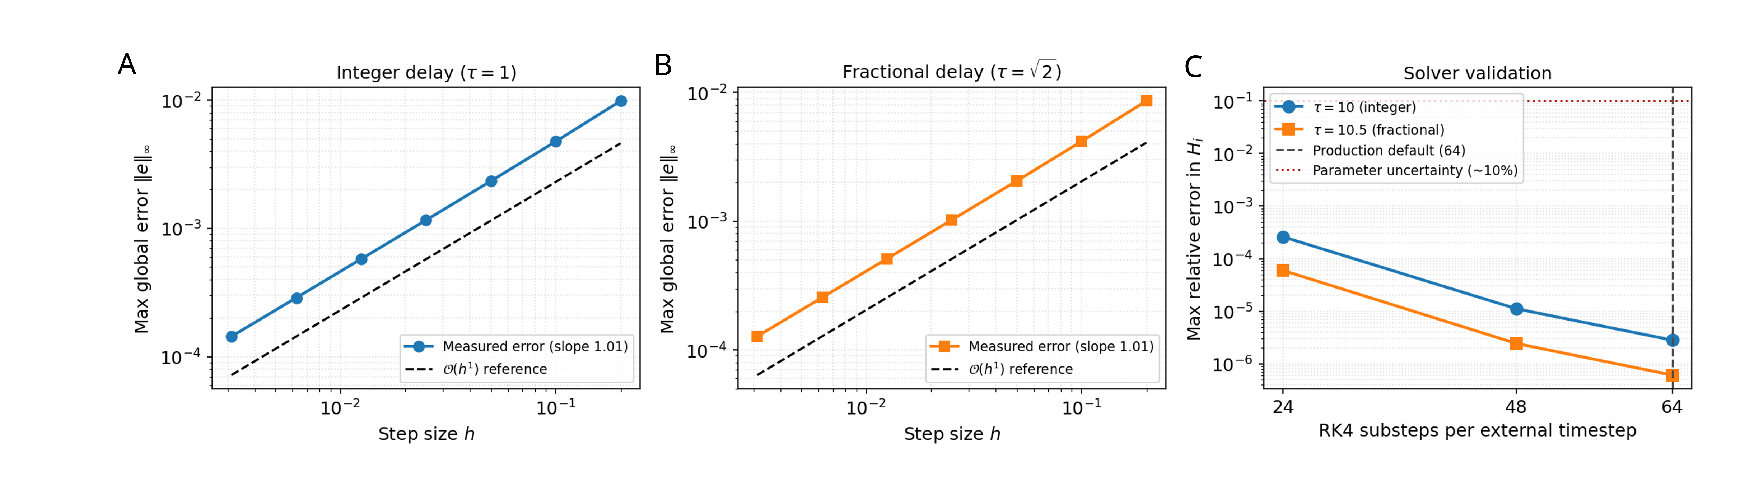
\includegraphics[width=\linewidth]{convergence_analysis.pdf}
    \caption{Convergence and solver validation of the frozen-delay RK4 scheme. (A)~Convergence on a scalar DDE with integer delay ($\tau = 1$) showing first-order global accuracy ($\mathcal{O}(h^1)$). (B)~Convergence with fractional delay ($\tau = \sqrt{2}$), confirming the same first-order rate when the interpolation code path is exercised. (C)~Production solver validation on the biological oscillator model: accumulated relative error in $H_i$ over 50 timesteps for 24, 48, and 64 RK4 substeps against a 96-substep reference trajectory. At the production value of 64 substeps, the relative error remains well below $10^{-4}$.}\label{fig:convergence}
\end{figure}

% ==========================================================
\section{Reservoir Architecture}
% ==========================================================

\subsection{Reservoir Size and Scaling}

Reservoir size $N$ was varied from 50 to 1000 nodes while holding all other parameters at the Phase~2 distance-topology best-trial values. The intended design was a single-fold grid over 10 unit counts; because the shared Optuna grid study was executed with concurrent workers, 25 completed evaluations were recorded, revisiting some grid points and providing limited repeat observations.

Classification accuracy increased up to approximately $N \approx 300$, beyond which performance entered a broad plateau. Under the fixed Phase~2-updated baseline, reservoir sizes from 250 to 1000 all remained viable, with the best observed single-fold result at $N = 300$. The main article reports the corresponding headline interpretation; Figure~\ref{fig:P1-units-slice} and the associated study tables are provided here for detailed inspection.

\begin{figure}[H]
    \centering
    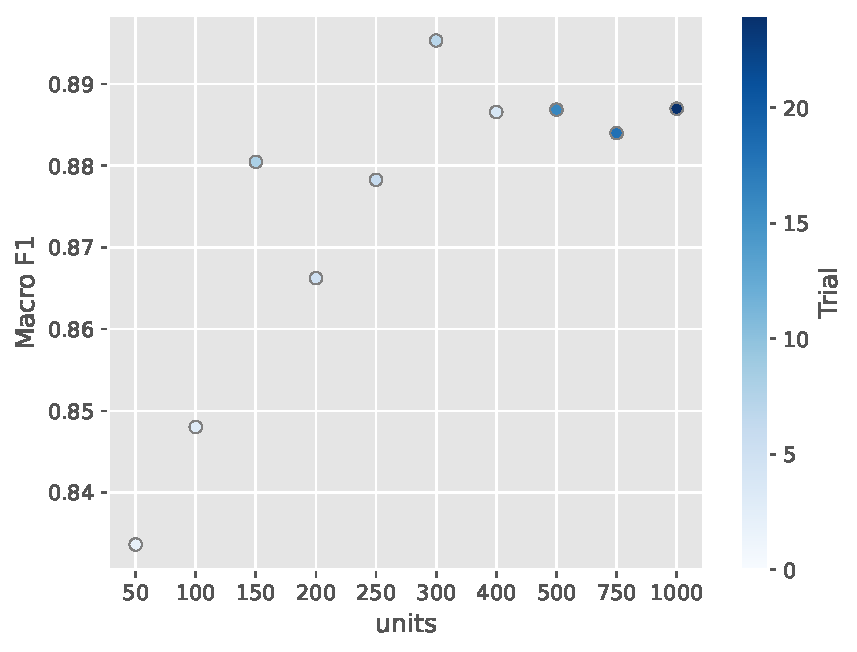
\includegraphics[width=0.85\linewidth]{P1-units-slice.pdf}
    \caption{Phase~1 sensitivity of classification performance to reservoir size (P1-units study). Macro F1 peaks around $N = 300$ and then remains on a broad plateau across larger reservoirs, indicating diminishing returns beyond moderate reservoir sizes under the fixed Phase~2-updated baseline.}\label{fig:P1-units-slice}
\end{figure}

\subsection{Input and Recurrent Gain Balance}

Input ($\alpha_u$) and recurrent ($\alpha_r$) scaling coefficients were varied over $10^{-4}$ to $10^{-2}$. Performance was primarily governed by the ratio $\alpha_u / \alpha_r$ rather than absolute magnitudes. Stable and high-performing regimes occurred when input-driven and recurrent contributions were of comparable order (see Figure~\ref{fig:P1-coupling-slice} and the corresponding scaling panels of the Phase~2 distance-topology joint optimization reported in the main article). Excessively large $\alpha_r$ produced self-sustained dynamics insensitive to input, whereas large $\alpha_u$ suppressed recurrent memory effects.

\subsection{DDE Input Coefficient}

The perturbation coefficient $\lambda$ was varied from $10^{-4}$ to $10^{-2}$. Values above $10^{-2}$ disrupted oscillatory stability, whereas values below $10^{-4}$ yielded insufficient input influence. The range $[2\times10^{-3}, 8\times10^{-3}]$ produced comparable performance (see the \texttt{dde\_scaling} panel in Figure~\ref{fig:P1-coupling-slice} and the corresponding Phase~2 distance-topology slice panels reported in the main article).

\subsection{Noise Sensitivity}

Input and recurrent noise levels were independently varied. Classification accuracy remained stable up to $\sigma_u = 0.05$ and $\sigma_r = 0.1$, beyond which performance degraded progressively (Figure~\ref{fig:P1-noise-slice}). This suggests moderate robustness to perturbations in stimulus delivery and coupling variability.

\subsection{State Representation}

Phase~1 screening found that reservoir states constructed from LuxI alone, or from the full $(A,I,H_i,H_e)$ vector per node, yielded statistically indistinguishable classification accuracy (paired t-test, $p > 0.05$) at $N = 250$ nodes. However, Phase~2 joint optimization selected $\{I, H_e\}$ (LuxI and extracellular AHL) as the observed output variables, providing a $2N$-dimensional feature vector. This shift reflects a parameter interaction: at the larger reservoir size ($N = 1000$) and co-adapted scaling coefficients identified during joint optimization, the additional $H_e$ features improved readout discrimination despite the higher feature dimensionality.

\subsection{Computational Scaling}

Runtime scaled approximately quadratically with $N$ prior to geometric cutoff, consistent with dense matrix multiplication. The imposed interaction radius reduced effective connectivity and improved scaling. To characterize pipeline costs at the production configuration ($N = 1000$), dedicated profiling runs were executed on Host~1 (Intel Xeon Gold 6538Y+, $2\times 64$ physical cores) with five folds running in parallel. Table~\ref{tab:pipeline-timings} reports per-stage mean wall-clock time per fold ($\pm$ std across five folds) for each headline task.

\begin{table}[H]
\centering
\caption{Pipeline profiling for the three biological headline tasks plus the ESN baseline (five-fold cross-validation, five parallel processes on Host~1). ``Train reservoir'' and ``Val reservoir'' denote reservoir-state generation for training and test instances respectively; ``Fit readout'' is classifier training on aggregated states; ``Predict'' includes readout inference plus evaluation. All times are per fold (mean $\pm$ std across five folds).}\label{tab:pipeline-timings}
\small
\begin{tabular}{lcccc}
\toprule
Pipeline Stage & Balanced 5-class & Binary & Unbalanced 5-class & ESN baseline \\
\midrule
Train Samples & 3215 & 30172 & 15307 & 3215 \\
Test Samples & 800 & 7542 & 800 & 800 \\
\midrule
Train reservoir & $232.0 \pm 1.7$\,s & $2150.0 \pm 2.0$\,s & $931.4 \pm 10.1$\,s & $77.2 \pm 1.1$\,s \\
Fit readout & $0.05 \pm 0.003$\,s & $377.0 \pm 2.0$\,s & $0.19 \pm 0.01$\,s & $1.66 \pm 0.08$\,s \\
Val reservoir & $56.9 \pm 0.4$\,s & $536.0 \pm 1.0$\,s & $231.1 \pm 1.7$\,s & $19.27 \pm 0.11$\,s \\
Predict & $14.1 \pm 0.3$\,s & $33.0 \pm 1.0$\,s & $123.9 \pm 4.2$\,s & $0.165 \pm 0.002$\,s \\
\midrule
Per-instance DDE & \multicolumn{4}{c}{$\approx 72$\,ms for the biological reservoir; not applicable to the ESN baseline} \\
\bottomrule
\end{tabular}
\end{table}

Reservoir simulation (DDE integration) dominates the biological pipeline, accounting for over 95\% of total wall time across all oscillator-reservoir tasks. The per-instance simulation cost of approximately \SI{72}{\milli\second} at $N = 1000$ nodes is consistent across balanced, binary, and unbalanced configurations, confirming that runtime scales linearly with instance count. Readout fitting is negligible for KNN ($< 0.2$\,s) but substantial for random forest (${\sim}377$\,s on $30{,}172$ instances) due to ensemble construction on a larger training set. The unbalanced task's fourfold increase in training time relative to the balanced task ($931$\,s vs.\ $232$\,s) is proportional to its fourfold larger training set ($12{,}886$ vs.\ $3{,}212$ instances), with no superlinear overhead. The ESN baseline completed the same balanced five-fold protocol in roughly 40\% of the balanced BioReservoir wall time, but at lower macro F1 ($0.878$ vs.\ $0.890$), making the runtime-performance tradeoff explicit. Total end-to-end wall time (five parallel folds on Host~1) was approximately 5 minutes for the balanced task, 52 minutes for the binary task (full balanced data), 22 minutes for the unbalanced task, and under 2 minutes for the ESN baseline. Inter-fold variance was low ($\sigma < 2\%$ of mean), indicating stable parallelization and negligible resource contention across folds.

% ==========================================================
\section{Hyperparameter Optimization --- Phase~1 Sensitivity Analysis}
% ==========================================================

\subsection{Optimization Framework and Computational Setup}

Hyperparameter optimization used Optuna~\cite{Akiba2019} with the Tree-structured Parzen Estimator (TPE) sampler for continuous and categorical parameters, and a grid sampler for the purely categorical normalization study. Studies were distributed across five dedicated servers (Table~\ref{tab:hardware}) running RHEL~9. Workers were allocated at half the available logical CPU count per host to maintain operating system headroom; each host ran 12--64 asynchronous parallel workers sharing a single SQLite-backed Optuna study file. Macro-averaged F1-score on the balanced five-class ECG classification task (803 samples per class, 4015 total) served as the primary objective. Weighted F1 was recorded in parallel for imbalanced result interpretation, but was not used for model selection. Each Phase~1 trial used a single stratified cross-validation fold (80/20 train/test split) as a computationally efficient proxy metric.

All experiments used Python~3.9.21 with the following key packages: reservoirpy~0.3.11, scikit-learn~1.5.0, NumPy~1.26.4, SciPy~1.13.0, Optuna~3.6.1, Numba~0.60.0, and joblib~1.4.2\@. Pinned dependency versions are tracked in a \texttt{requirements.txt} lockfile distributed with the code. All mathematical operations were computed using Numba with JIT compilation using CPU execution only.

Per-trial runtimes recorded during optimization studies were measured under heavy parallel load (12--64 concurrent workers per host) and therefore reflect wall-clock time under contention rather than isolated execution time. These values are useful for relative comparisons between studies and parameter configurations, but should not be interpreted as accurate single-trial runtimes. For headline results, we report runtimes from dedicated profiling runs using the \texttt{rerun-best} procedure with per-stage instrumentation (Table~\ref{tab:pipeline-timings}).

\begin{table}[H]
\centering
\caption{Hardware configuration of the five servers used for hyperparameter optimization. Workers were allocated at half the available logical CPU count per host.}\label{tab:hardware}
\small
\begin{tabular}{llcc}
\toprule
Host & Processor & Physical Cores & Memory (GB) \\
\midrule
Host~1 & Intel Xeon Gold 6538Y+ ($2\times$) & 64 & 1511 \\
Host~2 & Intel Xeon Silver 4516Y+ ($2\times$) & 48 & 754 \\
Host~3 & AMD EPYC 7302 ($2\times$) & 32 & 755 \\
Host~4 & Intel Xeon Silver 4410Y ($2\times$) & 24 & 251 \\
Host~5 & Intel Xeon Silver 4410Y & 12 & 125 \\
\bottomrule
\end{tabular}
\end{table}

\subsubsection*{Study Naming Convention}

Studies follow a phase-numbered naming scheme: a prefix \textbf{P1}--\textbf{P4} denotes the optimization phase, followed by a descriptive suffix identifying the parameter group or topology variant. Phase~1 sensitivity studies are prefixed \textbf{P1-} (e.g.\ \texttt{P1-scaling} for signal amplitude, \texttt{P1-topology-distance} for the distance-based topology). Phase~2 joint refinement studies use \textbf{P2-} with the topology type (\texttt{P2-distance}, \texttt{P2-random}). Phase~3 final configuration studies use \textbf{P3-} (\texttt{P3-imbalance}, \texttt{P3-binary}), and Phase~4 readout optimization studies use \textbf{P4-} (\texttt{P4-readout-balanced}, \texttt{P4-readout-binary}). We additionally use an \textbf{ESN-} prefix for the conventional leaky ESN comparator track (\texttt{ESN-balanced}, \texttt{ESN-readout}). Abbreviated forms (e.g.\ \texttt{P1-topo-dist}) are used in tables where space is limited.

Per-trial resource usage at $N = 250$ reservoir nodes was approximately \SI{400}{\mega\byte} resident set size (peak \SI{600}{\mega\byte}), with near single-core CPU utilization and wall-clock runtimes ranging from \SI{430}{\second} (input layer studies) to \SI{1250}{\second} (random topology construction, which requires full spectral radius normalization). A shared \emph{baseline} parameter set was held fixed in each study except for the group under investigation. After completing Phase~1, all baseline values were updated to the best-found values from each study before launching the Phase~2 joint refinement (Table~\ref{tab:phase1-best}).

\subsection{Study Overview}

Table~\ref{tab:study-overview} summarizes all 23 optimization studies conducted across the four BioReservoir phases, the ESN comparator track, and the no-reservoir baseline track. Completed trial counts may slightly exceed planned budgets because asynchronous workers atomically claim trials and may finish additional evaluations after the Optuna budget limit is reached; all completed trials are valid optimizer samples.

\begin{table}[H]
\centering
\caption{Complete optimization study overview across the four BioReservoir phases, the ESN comparator track, and the no-reservoir baseline track. Phase~1 studies isolate individual parameter groups (single-fold proxy); Phase~2 jointly optimizes all salient parameters (single-fold); Phase~3 evaluates the best configuration under alternative task settings (five-fold CV); Phase~4 optimizes the readout classifier on frozen reservoir states (five-fold CV); the ESN track applies the same training/readout workflow to a standard leaky ESN baseline; the Baseline track trains the same classifier families directly on raw z-scored ECG features without any reservoir transformation (five-fold CV). Best F1 is macro-averaged. Trial counts reflect completed evaluations.}\label{tab:study-overview}
\small
\begin{tabular}{llclccc}
\toprule
Phase & Study & Host & Parameter Group & Sampler & Trials & Best F1 \\
\midrule
\multirow{11}{*}{1}
 & P1-scaler        & 5 & Dataset normalization     & Grid & 21  & 0.760 \\
 & P1-scaling       & 2 & Signal amplitude scaling  & TPE  & 288 & 0.896 \\
 & P1-integration   & 3 & DDE integration           & TPE  & 128 & 0.816 \\
 & P1-topo-dist     & 1 & Distance topology         & TPE  & 256 & 0.836 \\
 & P1-topo-rand     & 1 & Random topology$^{a}$     & TPE  & 256 & 0.786 \\
 & P1-noise-data    & 5 & Data augmentation         & TPE  & 96  & 0.803 \\
 & P1-noise-res     & 4 & Reservoir noise           & TPE  & 144 & 0.795 \\
 & P1-input         & 4 & Input layer               & TPE  & 192 & 0.865 \\
 & P1-readout       & 2 & Readout aggregation       & TPE  & 191 & 0.783 \\
 & P1-units         & 2 & Reservoir size$^{b}$      & Grid & 25  & 0.895 \\
 & P1-coupling      & 3 & Cell coupling             & TPE  & 128 & 0.896 \\
\midrule
\multirow{2}{*}{2}
 & P2-distance      & 1 & Joint refined (distance)  & TPE  & 768 & 0.905 \\
 & P2-random        & 2 & Joint refined (random)    & TPE  & 800 & 0.907 \\
\midrule
\multirow{2}{*}{3}
 & P3-imbalance     & 1 & Class imbalance grid      & Grid & 5   & 0.921 \\
 & P3-binary        & 1 & Binary classification     & ---  & 1   & 0.931 \\
\midrule
\multirow{3}{*}{4}
 & P4-readout-bal.  & 4 & Balanced readout          & TPE  & 914  & 0.891 \\
 & P4-readout-unbal.& 2 & Unbalanced readout        & TPE  & 747  & 0.920 \\
 & P4-readout-bin.  & 3 & Binary readout            & TPE  & 1013 & 0.933 \\
\midrule
\multirow{2}{*}{ESN}
 & ESN-balanced     & 2 & Leaky ESN training        & TPE  & 240  & 0.879 \\
 & ESN-readout      & 4 & ESN frozen-state readout  & TPE  & 548  & 0.878 \\
\midrule
\multirow{3}{*}{Baseline$^{c}$}
 & B1-baseline      & 6 & Balanced 5-class (raw)    & TPE  & 367  & 0.886 \\
 & B2-baseline-unbal.& 7 & Unbalanced 5-class (raw) & TPE  & 333  & 0.916 \\
 & B3-baseline-bin. & 8 & Binary (raw)              & TPE  & 480  & 0.933 \\
\bottomrule
\end{tabular}
\vspace{0.4em}
\begin{flushleft}
\footnotesize
$^{a}$~Phase~1 baseline was calibrated under a distance-topology prior; an unbiased comparison is provided by Phase~2.
$^{b}$~P1-units used the Phase~2-updated baseline. The intended grid covered 10 unit counts once each, but 25 completed evaluations were recorded because concurrent workers revisited grid points in the shared Optuna study; see Figure~\ref{fig:P1-units-slice}\@. Phases~1 and~2 used a single stratified fold (1-fold), whereas Phases~3 and~4 used fivefold cross-validation.
Phase~4 studies optimized on frozen reservoir states and varied in trial count due to differing host capacity.
ESN-readout counts reflect completed trials at manuscript freeze; the profiled five-fold ESN rerun used the best available readout trial.
$^{c}$~Baseline studies trained classifiers directly on the raw z-scored 187-dimensional ECG feature vectors without any reservoir transformation, using the same five-fold stratified CV protocol, per-fold noise augmentation, and macro-F1 objective as the Phase~4 readout studies. Nine classifier families were searched (adding MLP and perceptron to the seven used in Phase~4). Trial counts reflect completed evaluations from 500 planned trials per study; studies were still running at manuscript freeze but had reached performance plateaus.
\end{flushleft}
\end{table}

\subsection{Standard ESN Comparator Track}

To test whether the biological reservoir's performance could be matched by a conventional reservoir under the same evaluation protocol, we ran a separate ESN comparator track using ReservoirPy's leaky ESN node. Study \texttt{ESN-balanced} optimized 11 ESN hyperparameters plus a conditional bias-scaling parameter over 240 completed TPE trials on the balanced five-class single-fold proxy task. The best ESN training trial (trial~239) achieved a macro F1-score of $0.879$ with $N = 850$ units, \texttt{tanh} activation, spectral radius $1.70$, leak rate $0.316$, recurrent connectivity $0.179$, input connectivity $0.625$, and low additive noise.

A follow-on frozen-state readout study, \texttt{ESN-readout}, completed 548 trials and selected a ridge classifier (trial~115; $\alpha = 4.11 \times 10^{-4}$, \texttt{fit\_intercept}=True, \texttt{solver}=\texttt{svd}). Applying that readout in a profiled five-fold rerun yielded $F_1 = 0.878 \pm 0.014$, accuracy $0.875$, MCC $= 0.846$, and $\kappa = 0.843$. This makes the ESN a credible comparator rather than a weak baseline: it approaches the BioReservoir result while remaining modestly below the distance-coupled oscillator reservoir.

\begin{figure}[H]
    \centering
    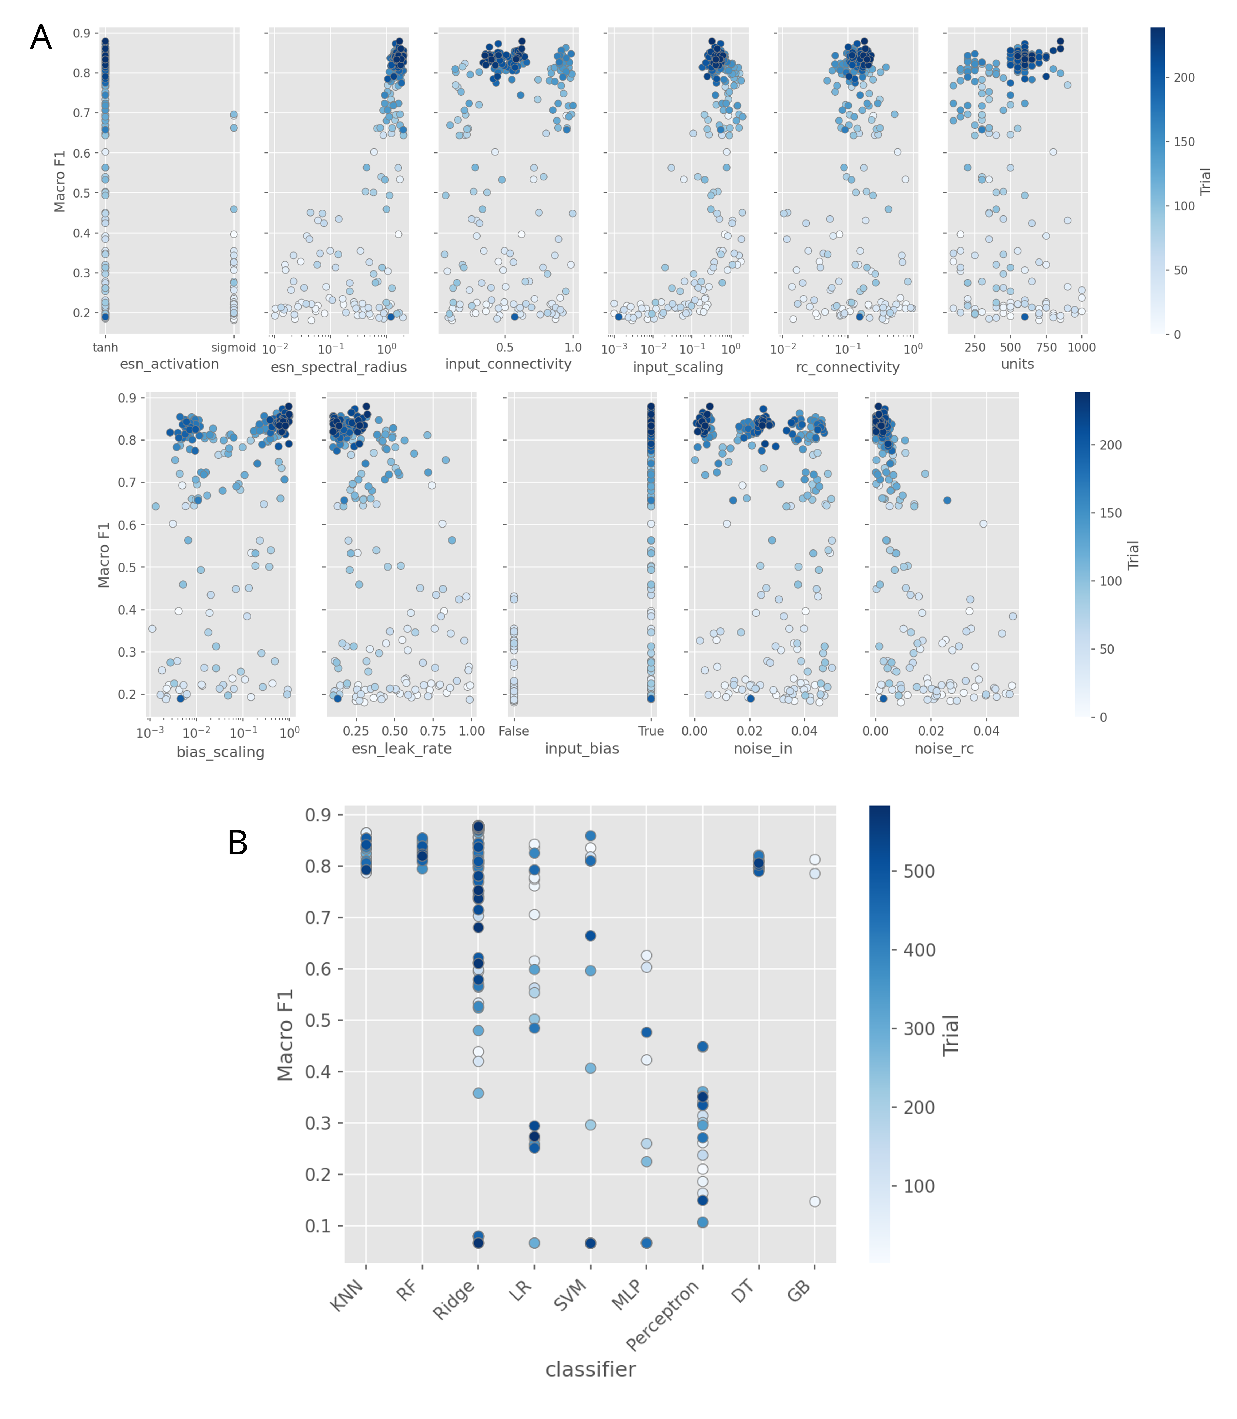
\includegraphics[width=1.0\linewidth]{ESN-training-readout-slice.pdf}
    \caption{Slice plots for the ESN comparator track. (A)~The ESN training study (\texttt{ESN-balanced}, 240 completed trials) shows that the top-performing region favors moderately large reservoirs, \texttt{tanh} activation, nonzero input bias, and intermediate recurrent connectivity. (B)~The frozen-state readout study (\texttt{ESN-readout}, 548 completed trials) is dominated by ridge configurations, consistent with the final five-fold ESN rerun.}\label{fig:esn-balanced-slice}
\end{figure}

\begin{table}[H]
\centering
\caption{Phase~1 best-trial parameter values adopted as the updated baseline for Phase~2 joint refinement. Baseline values are from preliminary iterative experiments; best values were identified by the corresponding sensitivity study.}\label{tab:phase1-best}
\small
\begin{tabular}{llllll}
\toprule
Parameter & Study & Baseline & Best Value & Search Range \\
\midrule
\texttt{scaler\_type} & P1-scaler & \texttt{seq\_zscore} & \texttt{seq\_zscore} & 6 strategies \\
\texttt{input\_scaling} & P1-scaling & $8.01 \times 10^{-2}$ & $1.03 \times 10^{-3}$ & $[10^{-4},\, 0.5]$ \\
\texttt{rc\_scaling} & P1-scaling & $1.95 \times 10^{-2}$ & $5.71 \times 10^{-4}$ & $[10^{-4},\, 0.2]$ \\
\texttt{dde\_scaling} & P1-scaling & $3.70 \times 10^{-3}$ & $7.46 \times 10^{-3}$ & $[5 \times 10^{-5},\, 0.02]$ \\
\texttt{rk4\_substeps} & P1-integration & 44 & 60 & $[12,\, 64]$ \\
\texttt{warmup} & P1-integration & 40 & 50 & $[10,\, 80]$ \\
\texttt{sparsity} & P1-topo-dist & 0.50 & 0.134 & $[0.05,\, 1.0]$ \\
\texttt{fade\_alpha} & P1-topo-dist & $1.81 \times 10^{-5}$ & $1.01 \times 10^{-6}$ & $[10^{-7},\, 10^{-2}]$ \\
\texttt{p\_excite} & P1-topo-dist & 0.50 & 0.66 & $[0.3,\, 0.7]$ \\
\texttt{signed} & P1-topo-dist & False & True & \{True, False\} \\
\texttt{cell\_coupling} & P1-coupling & 16.28 & 8.86 & $[0.01,\, 100]$ \\
\texttt{input\_connectivity} & P1-input & 0.19 & 0.368 & $[0.1,\, 1.0]$ \\
\texttt{output\_variables} & P1-input & \texttt{IHe} & \texttt{He} & 6 subsets \\
\texttt{readout\_aggregation} & P1-readout & \texttt{final} & \texttt{last\_N} & 3 strategies \\
\texttt{readout\_window} & P1-readout & 1 & 36 & $[1,\, 200]$ \\
\texttt{noise\_in} & P1-noise-res & $7.87 \times 10^{-2}$ & $1.44 \times 10^{-2}$ & $[0,\, 0.3]$ \\
\texttt{noise\_rc} & P1-noise-res & 0.121 & 0.240 & $[0,\, 0.3]$ \\
\texttt{noise\_rate} & P1-noise-data & $8.25 \times 10^{-2}$ & 0.300 & $[0,\, 0.3]$ \\
\texttt{noise\_ratio} & P1-noise-data & 0.235 & 0.286 & $[0,\, 0.3]$ \\
\bottomrule
\end{tabular}
\end{table}

\subsection{Dataset Normalization (P1-scaler)}

Six normalization strategies were evaluated using a grid sampler with five planned passes per strategy (30 trials total; 21 completed). Table~\ref{tab:P1-scaler} reports the best observed F1 per strategy. Per-sequence z-score normalization (\texttt{sequence\_zscore}) achieved the highest performance and was confirmed as the baseline scaler for all subsequent studies. Per-sequence strategies preserve the within-beat morphological shape while removing amplitude bias across beats, which is critical for discriminating arrhythmia classes that differ in waveform shape rather than absolute amplitude. Global strategies collapse inter-beat amplitude variation, discarding clinically relevant information. The margin between per-sequence z-score and global min/max normalization ($\Delta F_1 \approx 0.07$) confirms that beat-level normalization is essential for this task and justifies its use throughout.

\begin{figure}[H]
    \centering
    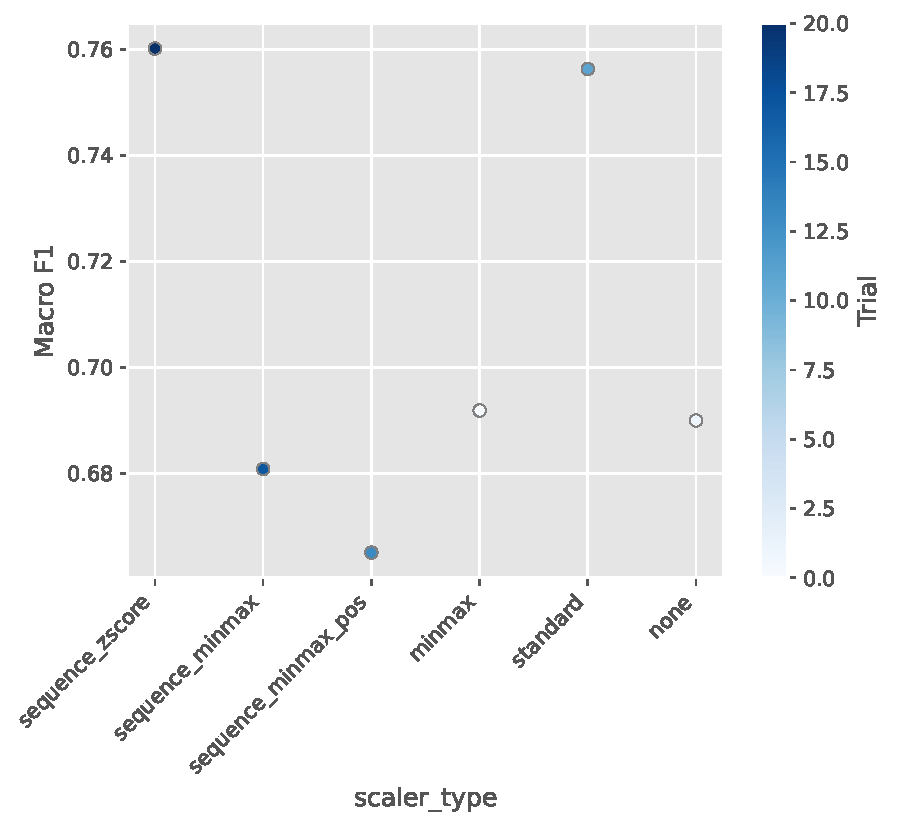
\includegraphics[width=0.85\linewidth]{P1-scaler-slice.pdf}
    \caption{Slice plot for the normalization strategy study (21 completed trials). Each vertical band corresponds to one normalization strategy; trial F1-scores confirm the clear advantage of per-sequence z-score normalization.}
    \label{fig:P1-scaler-slice}
\end{figure}

\begin{table}[H]
\centering
\caption{Classification performance by normalization strategy. Best macro F1 from completed trials is shown; 21 of 30 planned grid trials completed.}
\label{tab:P1-scaler}
\small
\begin{tabular}{lcc}
\toprule
Normalization Strategy & Best Macro F1 & Completed Trials \\
\midrule
\texttt{sequence\_zscore} (per-beat z-score) & 0.760 & 5 \\
\texttt{standard} (global z-score) & 0.756 & 6 \\
\texttt{minmax} (global min-max) & 0.692 & 1 \\
\texttt{none} (no normalization) & 0.690 & 1 \\
\texttt{sequence\_minmax} (per-beat min-max) & 0.681 & 4 \\
\texttt{sequence\_minmax\_pos} (per-beat min-max, non-negative) & 0.665 & 4 \\
\bottomrule
\end{tabular}
\end{table}

\subsection{Signal Amplitude Scaling (P1-scaling and P1-coupling)}

Two studies examined amplitude scaling parameters. The Phase~1 scaling study searched the three signal scaling coefficients governing input, recurrent, and DDE perturbation magnitudes; the Phase~1 coupling study jointly optimized inter-nodal coupling strength alongside the same three coefficients to characterize interactions between coupling and scaling. Search ranges and best values are shown in Table~\ref{tab:scaling}.

\begin{table}[H]
\centering
\caption{Search ranges and best trial values for signal scaling and coupling parameters. All continuous parameters were sampled on a log scale using TPE. Best F1 is reported per study.}
\label{tab:scaling}
\small
\begin{tabular}{lllccc}
\toprule
Parameter & Study & Search Range & Scale & Best Value & Best F1 \\
\midrule
\texttt{input\_scaling} & Phase~1 scaling & $[10^{-4},\ 0.5]$ & log & $1.03 \times 10^{-3}$ & \multirow{3}{*}{0.896} \\
\texttt{rc\_scaling} & Phase~1 scaling & $[10^{-4},\ 0.2]$ & log & $5.71 \times 10^{-4}$ & \\
\texttt{dde\_scaling} & Phase~1 scaling & $[5 \times 10^{-5},\ 2 \times 10^{-2}]$ & log & $7.46 \times 10^{-3}$ & \\
\midrule
\texttt{cell\_coupling} & Phase~1 coupling & $[10^{-2},\ 10^{2}]$ & log & 8.86 & \multirow{4}{*}{0.896} \\
\texttt{input\_scaling} & Phase~1 coupling & $[10^{-4},\ 10^{-1}]$ & log & $5.65 \times 10^{-2}$ & \\
\texttt{rc\_scaling} & Phase~1 coupling & $[10^{-4},\ 10^{-1}]$ & log & $2.78 \times 10^{-2}$ & \\
\texttt{dde\_scaling} & Phase~1 coupling & $[10^{-4},\ 10^{-2}]$ & log & $4.32 \times 10^{-4}$ & \\
\bottomrule
\end{tabular}
\end{table}

The scaling parameters selected by the Phase~1 scaling study differed substantially from the preliminary baseline (input and recurrent scaling decreased by approximately 2.0 and 1.5 orders of magnitude, respectively), confirming that the reservoir operates in a low-amplitude input regime in which DDE dynamics are gently perturbed rather than driven to saturation. The Phase~1 coupling study confirmed that \texttt{cell\_coupling} is a genuine free parameter: at \texttt{cell\_coupling}~$= 8.86$, the top-of-range basin differs from the single-factor optimum identified by the scaling-only study, indicating interactions between coupling and scaling that motivate joint refinement in Phase~2. Notably, seven of the top ten coupling-study trials clustered in $\texttt{cell\_coupling} \in [8, 30]$, suggesting a broad but well-defined optimal region.

\begin{figure}[H]
    \centering
    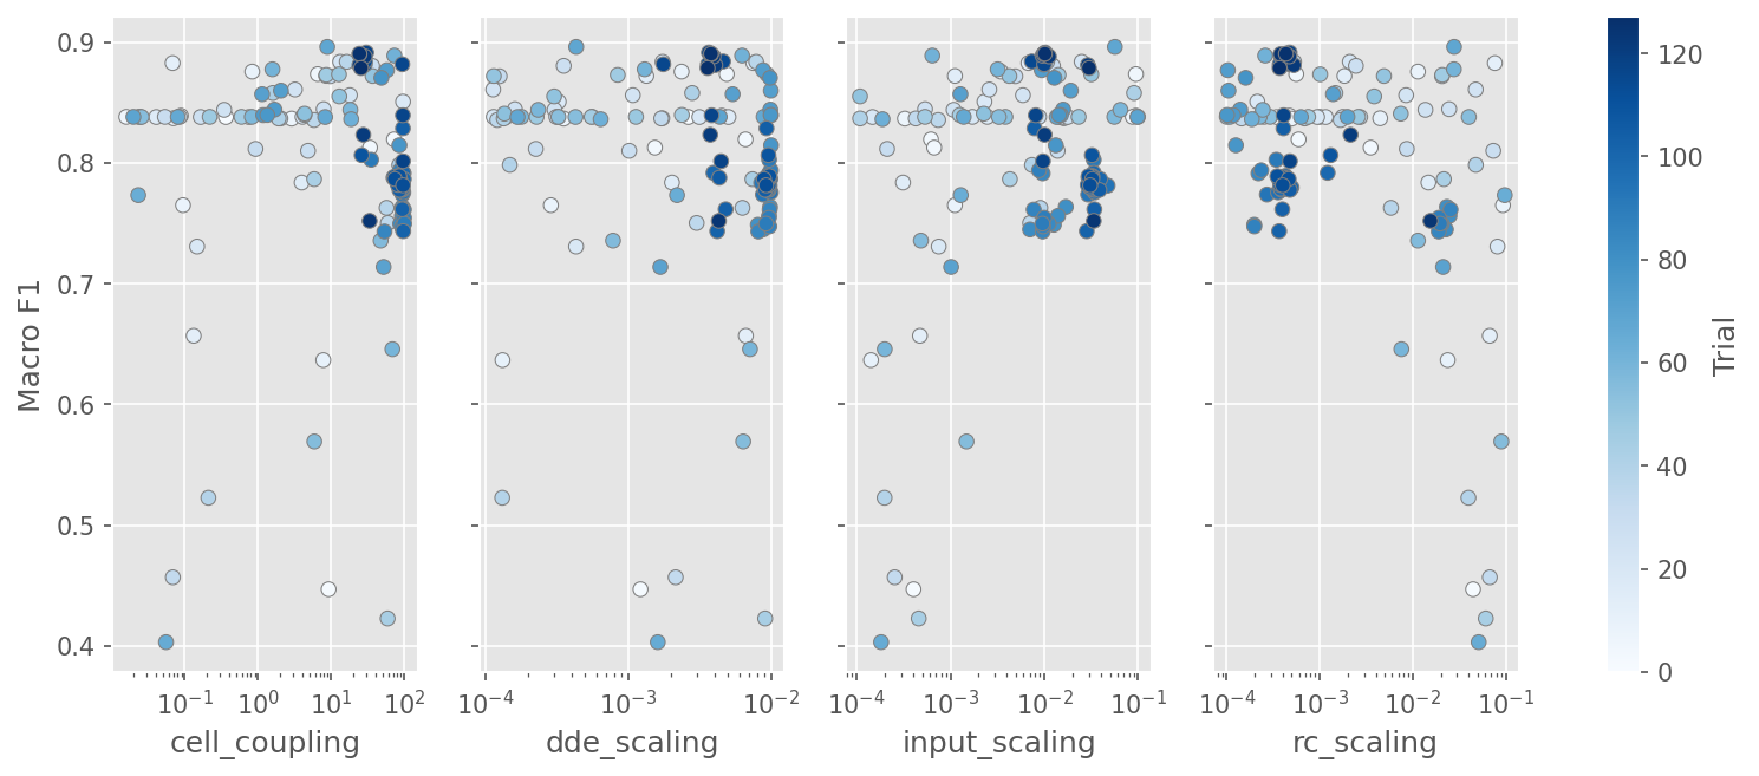
\includegraphics[width=0.82\linewidth]{P1-coupling-slice.pdf}
    \caption{Slice plot for the Phase~1 coupling study. Joint variation of coupling strength with the three scaling coefficients reveals a broad high-performing basin at \texttt{cell\_coupling} $\in [8, 30]$, confirming that interactions between coupling and scaling motivate joint refinement in Phase~2.}
    \label{fig:P1-coupling-slice}
\end{figure}

\subsection{DDE Integration Parameters (P1-integration)}

Study P1-integration examined the RK4 substep count per external timestep (\texttt{rk4\_substeps}, $\{12, \ldots, 64\}$, step 4) and zero-input warmup duration (\texttt{warmup}, $\{10, \ldots, 80\}$, step 5). The best trial achieved $F_1 = 0.816$ at \texttt{rk4\_substeps}~$= 60$ and \texttt{warmup}~$= 50$. Both values reached the upper boundary of their search intervals, indicating that further performance improvements may be achievable at higher substep counts. Accordingly, the \texttt{rk4\_substeps} ceiling was extended to 88 for Phase~2. The top-performing warmup values clustered at $\{50, 80\}$ timesteps, with the 40-timestep baseline appearing rarely in the top trials, confirming that transient initialization dynamics require at least 50 timesteps to dissipate and that the prior warmup of 40 was marginally suboptimal.

\begin{figure}[H]
    \centering
    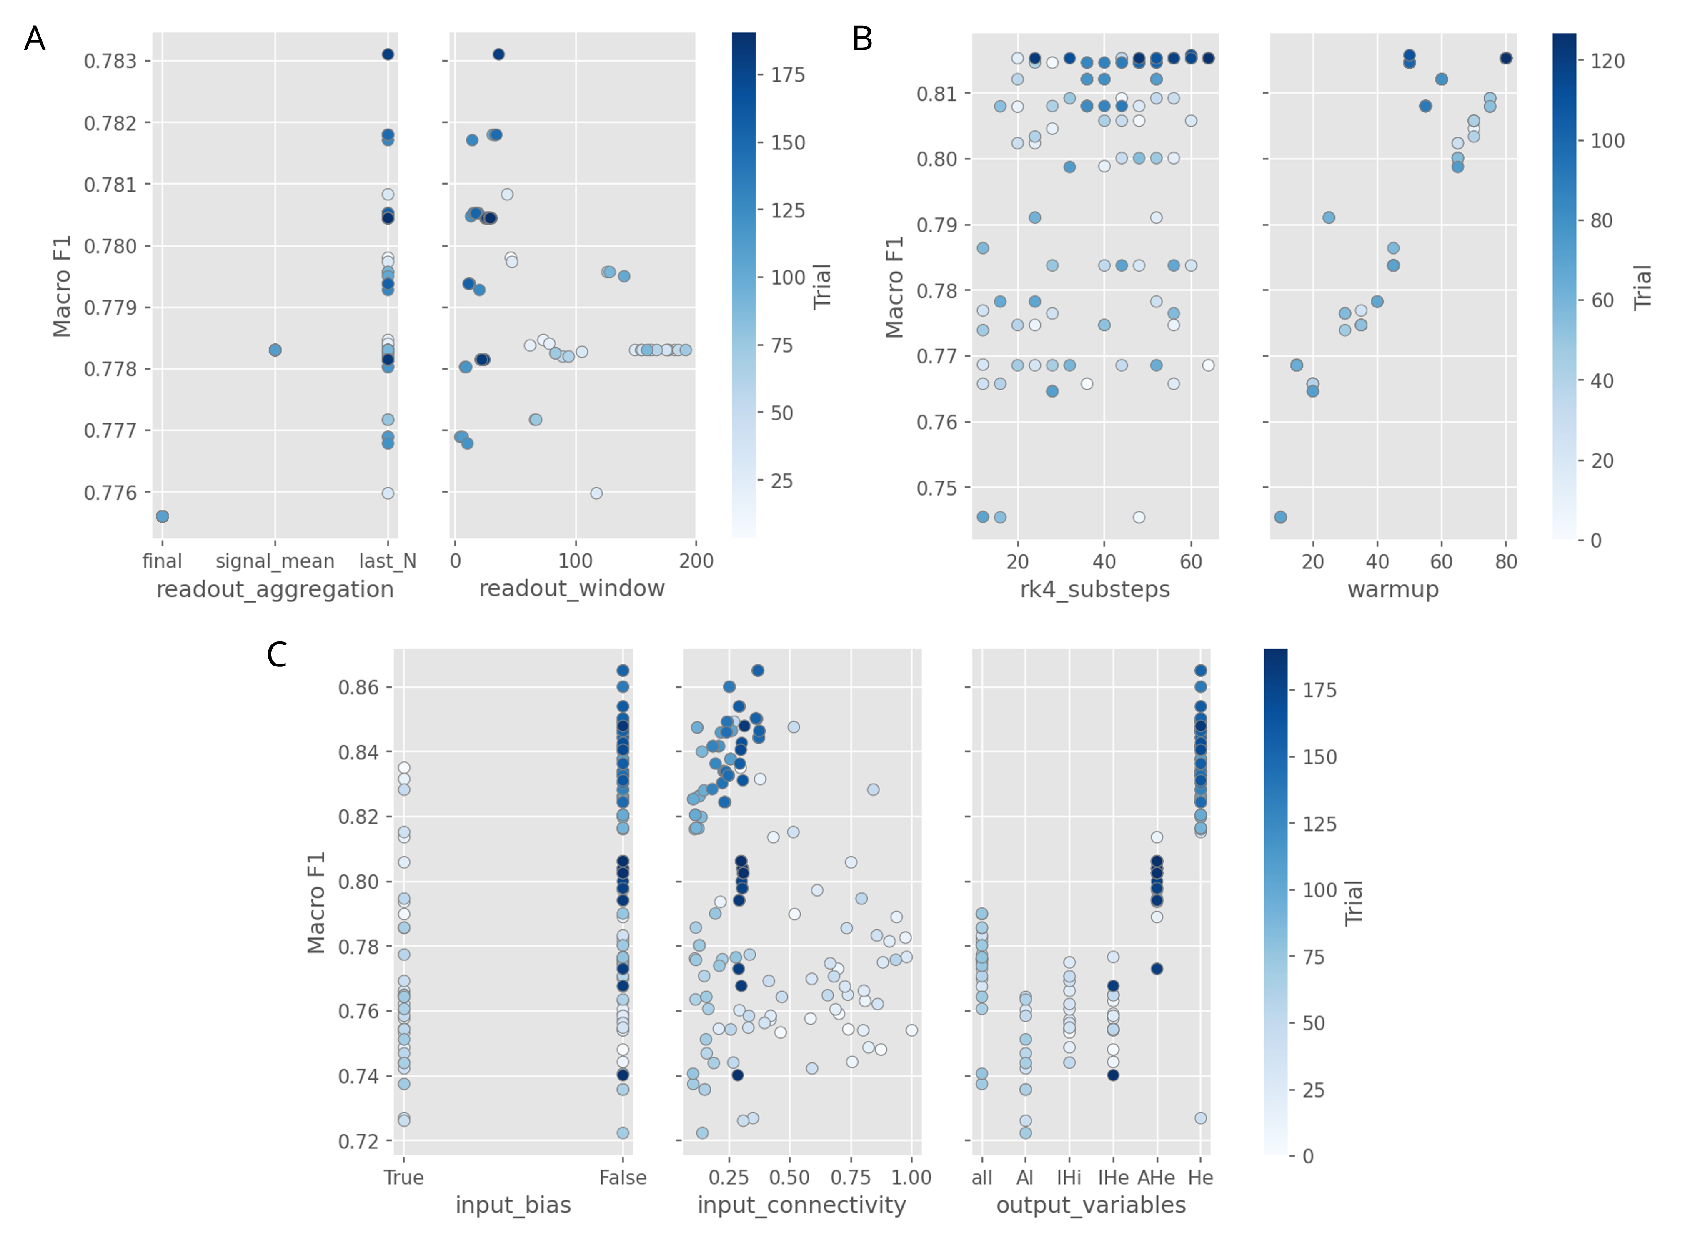
\includegraphics[width=0.9\linewidth]{P1-readout-integration-input.pdf}
    \caption{Phase~1 sensitivity slice plots for readout aggregation, DDE integration, and input-layer studies. (A)~P1-readout shows that temporal aggregation over the last 36 timesteps substantially outperforms single-timestep readout. (B)~P1-integration reaches the upper boundary of the search range, prompting an extended ceiling in Phase~2. (C)~P1-input shows that $H_e$ alone outperforms multi-variable state representations at $N = 250$.}\label{fig:P1-readout-integration-input}
\end{figure}

\subsection{Reservoir Topology (P1-topology-distance and P1-topology-random)}

Two topology studies were deployed simultaneously on the same server (Host 1, 128 cores, 64 workers each). Study P1-topo-dist optimized four parameters of the biologically motivated distance-based coupling kernel; study P1-topo-rand optimized three parameters of a random Gaussian topology. Table~\ref{tab:topology} reports search ranges and best-trial values.

\begin{table}[H]
\centering
\caption{Search ranges and best-trial values for topology parameters (P1-topo-dist: distance-based; P1-topo-rand: random Gaussian).}\label{tab:topology}
\footnotesize
\begin{tabular}{lllccc}
\toprule
Parameter & Study & Search Range & Scale & Best Value & Best F1 \\
\midrule
\texttt{sparsity} & P1-topo-dist & $[0.05,\ 1.0]$ & uniform & 0.134 & \multirow{4}{*}{0.836} \\
\texttt{fade\_alpha} & P1-topo-dist & $[10^{-7},\ 10^{-2}]$ & log & $1.01 \times 10^{-6}$ & \\
\texttt{p\_excite} & P1-topo-dist & $[0.3,\ 0.7]$ & uniform & 0.66 & \\
\texttt{signed} & P1-topo-dist & \{True, False\} & categorical & True & \\
\midrule
\texttt{rc\_connectivity} & P1-topo-rand & $[0.05,\ 1.0]$ & uniform & 0.397 & \multirow{3}{*}{0.786} \\
\texttt{p\_excite} & P1-topo-rand & $[0.3,\ 0.7]$ & uniform & 0.314 & \\
\texttt{signed} & P1-topo-rand & \{True, False\} & categorical & True & \\
\bottomrule
\end{tabular}
\end{table}

The distance topology achieved $F_1 = 0.836$ vs.\ $0.786$ for the random topology under Phase~1 conditions. However, this comparison is confounded by the Phase~1 baseline: scaling coefficients and coupling strength had been iteratively refined using the distance topology as the default, providing an inherent parametric advantage to the Phase~1 distance-topology study. An unbiased comparison is provided by the Phase~2 distance and random-topology studies, which independently optimize all parameters for each topology under an identical trial budget and search space. Both studies identified \texttt{signed}~$=$~True as optimal, indicating that mixed excitatory and inhibitory connectivity outperforms purely excitatory coupling regardless of topology type. The best Phase~1 distance-topology trial used a highly sparse weight matrix (active density 0.134) and very slow decay (\texttt{fade\_alpha}~$= 10^{-6}$), implying effective long-range interactions within the unit-square spatial domain.

Although P1-topo-rand nominally searched three parameters, parameter importance analysis identified only two as informative: \texttt{rc\_connectivity} (53\%) and \texttt{signed} (47\%).
The third parameter, \texttt{p\_excite}, controls the ratio of excitatory to inhibitory edges and is only meaningful when \texttt{signed}~$=$~True; when \texttt{signed}~$=$~False all weights are positive and \texttt{p\_excite} has no effect. Accordingly, the TPE sampler allocated 184 of 256 trials to \texttt{signed}~$=$~True, where performance varied with the continuous parameters, and 72 trials to \texttt{signed}~$=$~False, where all trials achieved an identical $F_1 = 0.732$ regardless of \texttt{p\_excite} or \texttt{rc\_connectivity}. The slice plot for the Phase~1 random-topology study therefore shows only the two informative parameters (Figure~\ref{fig:P1-topology-slice}B).

\begin{figure}[H]
    \centering
    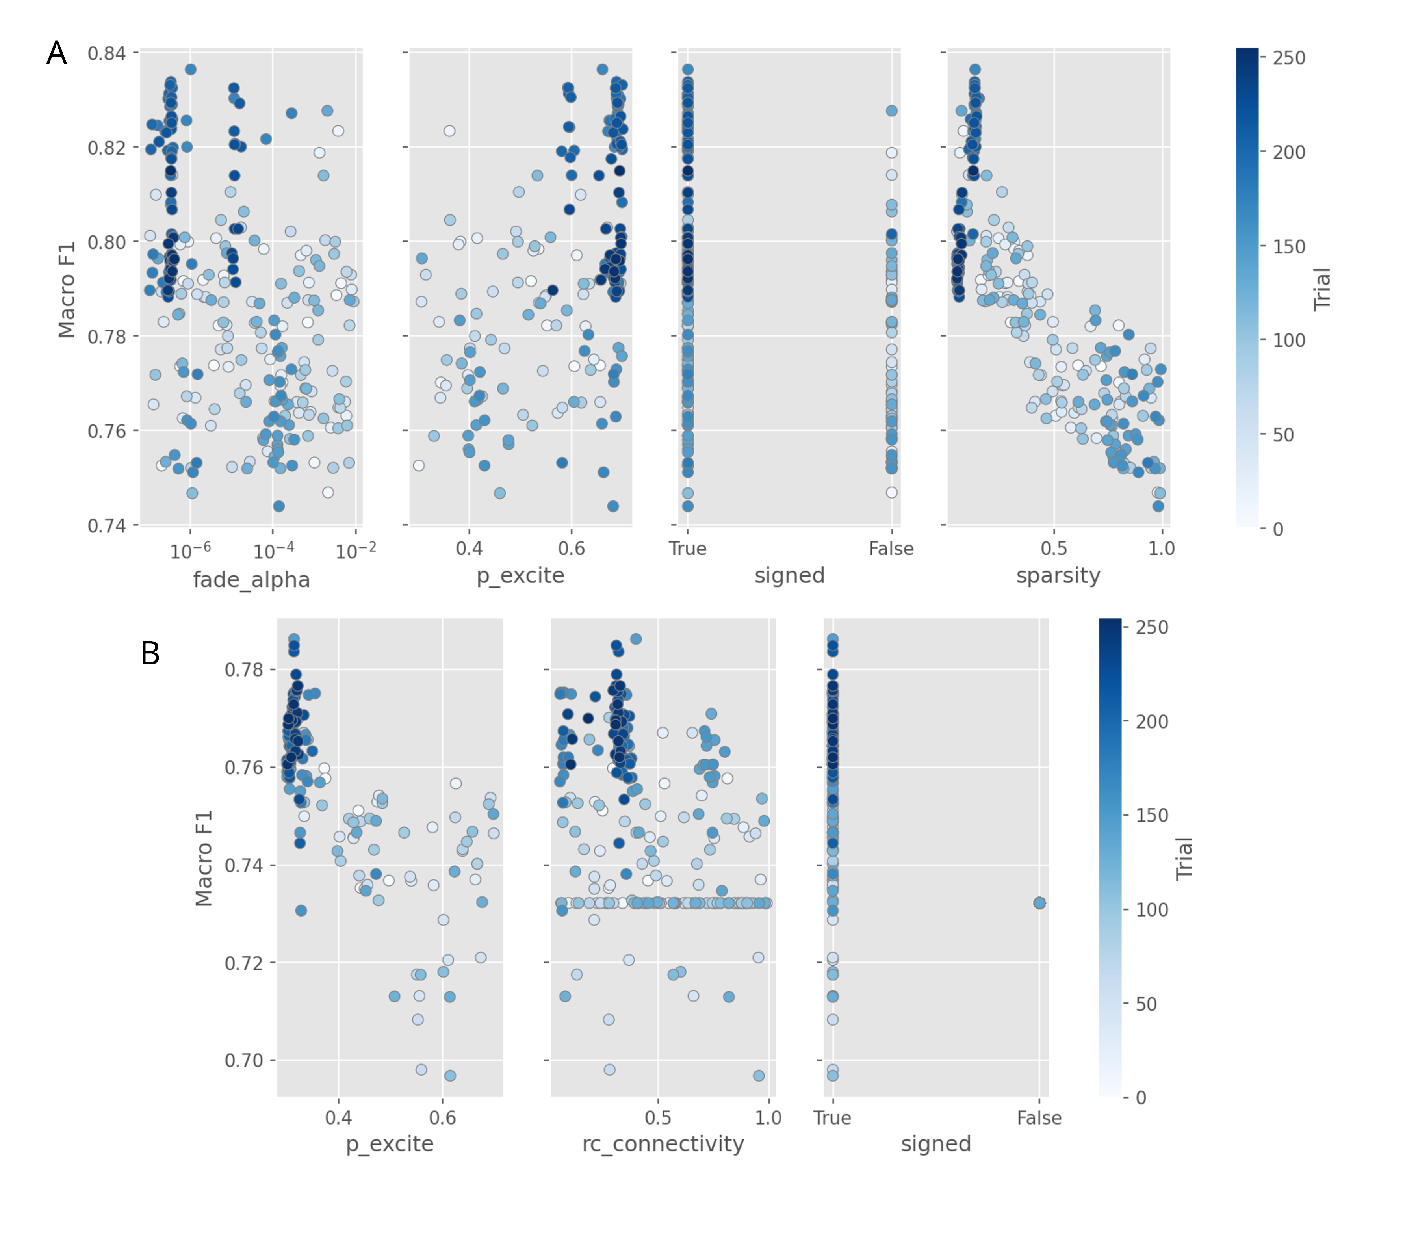
\includegraphics[width=0.8\linewidth]{P1-topology-combined.pdf}
    \caption{Slice plots for reservoir topology studies. (A)~The distance-based topology favors sparse connectivity (\texttt{sparsity}~$= 0.134$) with slow spatial decay. (B)~The random topology achieves lower peak F1 under Phase~1 conditions; this gap narrows under independent joint optimization in Phase~2.}\label{fig:P1-topology-slice}
\end{figure}

\subsection{Input Layer and Output Variables (P1-input)}

Study P1-input searched three input layer parameters: the fraction of reservoir nodes receiving input (\texttt{input\_connectivity} $\in [0.1, 1.0]$), the presence of an input bias (\texttt{input\_bias} $\in \{$True, False$\}$, with conditional \texttt{fixed\_bias\_scaling} $\in [10^{-4}, 0.1]$ log-scale when True), and the reservoir state variables observed by the readout (\texttt{output\_variables} $\in \{$all, AI, IHi, IHe, AHe, He$\}$). Best values were \texttt{input\_connectivity}~$= 0.368$, \texttt{input\_bias}~$= $~False, and \texttt{output\_variables}~$= $~\texttt{He} ($F_1 = 0.865$).

The selection of the extracellular AHL concentration ($H_e$) alone as the readout feature is notable: it provided the best performance while contributing only $N = 250$ features (vs.\ $2N = 500$ for \texttt{IHe}, $4N = 1000$ for all state variables). This indicates that the $k$-nearest neighbors readout benefits substantially from reduced feature dimensionality at $N = 250$ nodes, consistent with the curse of dimensionality for distance-based classifiers. From an experimental translation standpoint, this is a favorable constraint: measuring a single extracellular quantity per node (e.g., AHL concentration via a coupled fluorescent reporter such as sfGFP) is vastly more achievable than multiplexing four intracellular reporters, reducing the required imaging complexity to a single fluorescence channel. The top-10 trials clustered in \texttt{input\_connectivity}~$\in [0.25, 0.37]$, suggesting a saturation effect above 0.37; full connectivity ($= 1.0$, the prior baseline) was not present among the top-performing trials.

\subsection{Readout Aggregation Strategy (P1-readout)}

Study P1-readout evaluated three strategies for collapsing the reservoir state time-series to a fixed-dimensional feature vector for the readout: (i)~\texttt{final}, using only the reservoir state at the last input timestep; (ii)~\texttt{signal\_mean}, averaging over all signal-duration timesteps; and (iii)~\texttt{last\_N}, averaging over the last $K$ timesteps, with $K \in [1, 200]$ as a conditional parameter. All 191 completed trials included \texttt{last\_N} in the top-10 results, with best window $K = 36$ ($F_1 = 0.7831$). The \texttt{final} strategy did not appear in the top 10, with all \texttt{final} trials scoring below $F_1 = 0.780$.

This finding corrected a substantive error in the Phase~1 baseline: the baseline had assumed \texttt{final} as the default aggregation based on preliminary results, but P1-readout demonstrated that a 36-timestep averaging window consistently outperforms single- timestep readout. The baseline was updated to \texttt{last\_N} with $K = 36$ for Phase~2. The Phase~1 absolute performance values in Table~\ref{tab:study-overview} therefore underestimate the Phase~2 achievable performance for the other Phase~1 studies, which were all run with the suboptimal \texttt{final} aggregation baseline.

\subsection{Data Augmentation and Reservoir Noise (P1-noise-data and P1-noise-reservoir)}

Study P1-noise-data optimized two augmentation parameters: the noise amplitude relative to the per-sequence standard deviation (\texttt{noise\_rate} $\in [0.0, 0.3]$) and the fraction of each class's training samples to augment (\texttt{noise\_ratio} $\in [0.0, 0.3]$). Best values were \texttt{noise\_rate}~$= 0.300$ and \texttt{noise\_ratio}~$= 0.286$ ($F_1 = 0.803$); both values lay near the upper boundary of the search range, suggesting that augmentation amplitude and coverage monotonically improve classification F1 within the interval searched. Study P1-noise-reservoir optimized additive Gaussian noise injected at the input (\texttt{noise\_in} $\in [0.0, 0.3]$) and recurrent connections (\texttt{noise\_rc} $\in [0.0, 0.3]$) per timestep. Best values were \texttt{noise\_in}~$= 0.014$ and \texttt{noise\_rc}~$= 0.240$ ($F_1 = 0.795$).

Both noise studies exhibited modest absolute performance ($F_1 \approx 0.79$--$0.80$) relative to the scaling and input studies, confirming that noise parameters are weak levers in this architecture. Their best-trial F1 values lie close to the baseline performance of the fixed configuration, with noise acting as a mild regularizer rather than a major performance determinant. Best-trial values were nonetheless incorporated into the Phase~2 baseline for completeness.

\begin{figure}[H]
    \centering
    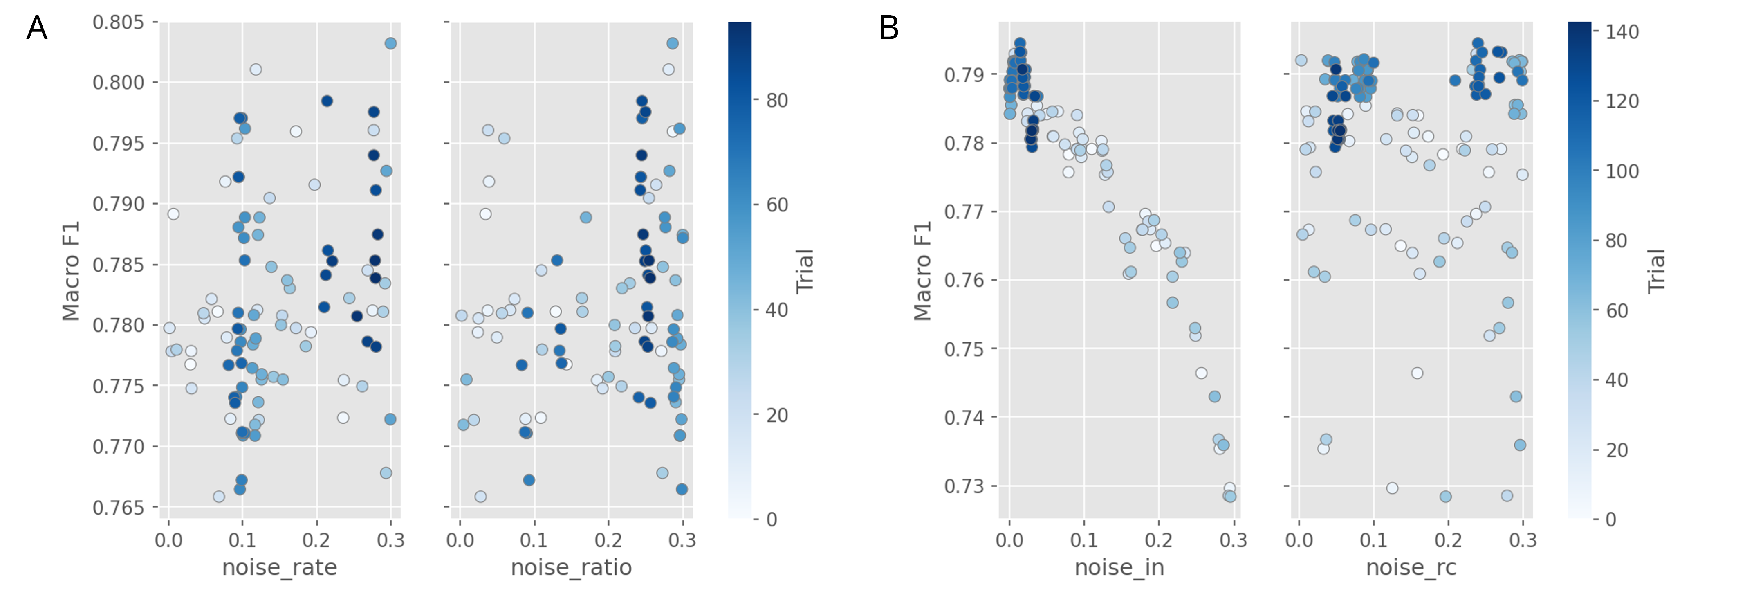
\includegraphics[width=\linewidth]{P1-noise-dataset-reservoir.pdf}
    \caption{Slice plots for noise studies. Both studies exhibit flat F1 landscapes near the baseline, confirming that noise parameters are weak performance levers. (A)~Data augmentation rate and amplitude both reach the upper boundary. (B)~Reservoir noise studies show modest recurrent noise ($\sigma_r \approx 0.24$) as mildly beneficial.}\label{fig:P1-noise-slice}
\end{figure}


% ==========================================================
\section{Dataset Characteristics and Preprocessing}

\subsection{Dataset Overview}

All experiments used the MIT-BIH Arrhythmia Database~\cite{Moody2001} in the pre-segmented form released by Kachuee et al.~\cite{Kachuee2018}. In the CSV release used here, the working dataset contains 109,446 single-heartbeat ECG segments sampled at 125\,Hz with 187 samples per beat ($\approx$1.5\,s per beat). Kachuee et al. grouped beats into five heartbeat classes in accordance with the AAMI EC57 standard: Normal~(N), Supraventricular ectopic~(S), Ventricular ectopic~(V), Fusion~(F), and Unknown~(Q). The raw class distribution is shown in Table~\ref{tab:raw-class-dist}; three task configurations were evaluated, with per-class counts through the preprocessing pipeline shown in Table~\ref{tab:per-class-pipeline}.

Preprocessing first determines per-class sample counts for the cross-validation (CV) pool; the pool is then evaluated by stratified five-fold CV (\texttt{StratifiedKFold}), which splits each fold into ${\approx}80\%$ training and ${\approx}20\%$ test while preserving class proportions. For the balanced five-class task, each class was limited to the smallest class size (803 samples per class), giving an equal-representation pool of 4\,015 instances; because all classes are equally sized, each fold's test set is approximately balanced (${\approx}$161 samples per class). For the unbalanced task, the per-class cap was raised to $5\times$ (4\,015); each class contributes up to the cap or its available count, whichever is smaller, yielding a pool of 16\,107 instances. Stratified splitting preserves the unequal class proportions in each fold, so per-fold test counts vary (e.g., ${\approx}$835 for Normal vs.\ ${\approx}$161 for Fusion); because the primary metric (macro F1) weights all classes equally, this proportional test composition does not bias the headline result. For binary classification, all non-Normal classes were merged into a single Arrhythmia category and both classes were balanced to the smallest merged class size (18\,857), giving a pool of 37\,714 instances with ${\approx}$3\,771 test samples per fold. All stochastic procedures (splitting, shuffling, augmentation, reservoir initialization) used a fixed random seed (6337) for full reproducibility.

\begin{table}[H]
\centering
\caption{Raw class distribution in the Kachuee MIT-BIH dataset.}
\label{tab:raw-class-dist}
\small
\begin{tabular}{lrr}
\toprule
Class & Count & Percentage \\
\midrule
Normal (N) & 90\,589 & 82.8\% \\
Supraventricular (S) & 2\,779 & 2.5\% \\
Ventricular (V) & 7\,236 & 6.6\% \\
Fusion (F) & 803 & 0.7\% \\
Unknown (Q) & 8\,039 & 7.3\% \\
\midrule
Total & 109\,446 & 100\% \\
\bottomrule
\end{tabular}
\end{table}

\begin{table}[H]
\centering
\caption{Approximate per-fold instance counts for all three tasks under stratified five-fold cross-validation. Each task's CV pool is first assembled by limiting per-class counts (see text), then \texttt{StratifiedKFold} splits each fold into ${\approx}80\%$ training and ${\approx}20\%$ test, preserving class proportions. ``Train'' is the pre-augmentation per-fold training count; ``Train+Aug'' includes noise-augmented copies appended per fold (see Section~\ref{sec:si-noise-augmentation}). The CV pool is the full pre-augmentation dataset supplied to cross-validation. For the balanced task all five classes contribute equally (803 each); for the unbalanced task larger classes contribute more instances, so per-fold test counts vary by class. For binary, all non-Normal classes are merged into Arrhythmia and both classes are balanced to the smallest merged class size (18\,857). Values are rounded to the nearest integer; exact counts vary by $\pm 1$ across folds due to integer partitioning.}\label{tab:per-class-pipeline}\footnotesize % chktex 24
\begin{tabular}{l rrr rrr rrr} % chktex 24
\toprule
& \multicolumn{3}{c}{Balanced 5-class} & \multicolumn{3}{c}{Unbalanced 5-class} & \multicolumn{3}{c}{Binary} \\
\cmidrule(lr){2-4} \cmidrule(lr){5-7} \cmidrule(lr){8-10}
Class & Train & Train+Aug & Test & Train & Train+Aug & Test & Train & Train+Aug & Test \\
\midrule
N & 643 & 827 & 160 & 3\,340 & 4\,295 & 835 & 15\,086 & 19\,403 & 3\,771 \\
S & 643 & 827 & 160 & 2\,223 & 2\,859 & 556 & --- & --- & --- \\
V & 643 & 827 & 160 & 3\,340 & 4\,295 & 835 & --- & --- & --- \\
F & 643 & 827 & 160 & 642 & 825 & 161 & --- & --- & --- \\
Q & 643 & 827 & 160 & 3\,340 & 4\,295 & 835 & --- & --- & --- \\
Arr. & --- & --- & --- & --- & --- & --- & 15\,086 & 19\,403 & 3\,771 \\
\midrule
Total & 3\,215 & 4\,135 & 800 & 12\,885 & 16\,569 & 3\,222 & 30\,172 & 38\,806 & 7\,542 \\
CV pool & \multicolumn{3}{c}{4\,015} & \multicolumn{3}{c}{16\,107} & \multicolumn{3}{c}{37\,714} \\
\bottomrule
\end{tabular}
\end{table}

\subsection{Normalization}

Per-sequence z-score normalization was applied in all experiments:
\begin{equation}
\tilde{x}_t = \frac{x_t - \mu_x}{\sigma_x},
\end{equation}
where $\mu_x$ and $\sigma_x$ are the mean and standard deviation of the individual sequence. Because statistics are computed independently per sequence, no test-set information influences training. The selection of per-sequence z-score over five alternative strategies was validated by the Phase~1 normalization study (Figure~\ref{fig:P1-scaler-slice}).

\subsection{Noise Augmentation}\label{sec:si-noise-augmentation}

Additive Gaussian noise augmentation was applied to a randomly selected subset of each class's training samples. For each selected sample, a noisy copy was generated as:
\begin{equation}
x_t^{\text{aug}} = x_t + \epsilon_t, \quad \epsilon_t \sim \mathcal{N}(0, \eta^2 \sigma_x^2),
\end{equation}
where $\eta = 0.300$ is the noise rate (fraction of per-sequence standard deviation used as noise amplitude) and $\sigma_x$ is the standard deviation of the original sequence. Approximately $28.6\%$ of each class's training samples (\texttt{noise\_ratio} $= 0.286$) were selected for augmentation; noisy copies were appended to the training set only. Both augmentation parameters were determined by the Phase~1 data augmentation study (P1-noise-data; Table~\ref{tab:phase1-best}).
% ==========================================================



% ==========================================================
\section{Classification Workflow and Algorithmic Implementation}

\subsection{Cross-Validation Procedure}

Model evaluation was performed using stratified five-fold cross-validation. For each fold, the dataset was partitioned into training (80\%) and validation (20\%) subsets while preserving class distributions. Noise augmentation was applied exclusively to the training subset.

The classification procedure is summarized below:

\begin{verbatim}
CROSS-VALIDATE(X, Y, reservoir, readout, k):
    folds = stratified_k_fold_split(X, Y, k)
    fold_metrics = []

    FOR EACH (X_train, Y_train, X_val, Y_val) IN folds:
        X_train = augment(X_train)
        X_train, X_val = normalise(X_train, X_val)

        train_states = reservoir.run(X_train)
        readout.fit(train_states, Y_train)

        val_states = reservoir.run(X_val)
        Y_pred = readout.predict(val_states)

        fold_metrics.append(evaluate(Y_val, Y_pred))

    RETURN mean(fold_metrics)
\end{verbatim}

\subsection{Reservoir State Extraction}

Each ECG instance was processed independently:

\begin{verbatim}
RESERVOIR.RUN(X):
    states = []
    FOR EACH instance IN X:
        reset_reservoir_state()
        state = integrate_dde(reservoir_weights, instance, dt)
        states.append(final_state)
    RETURN states
\end{verbatim}

Reservoir weights were fixed and identical across folds. Only the readout parameters were optimized.
% ==========================================================


% ==========================================================
\section{Hyperparameter Optimization --- Phase~2 Joint Refinement}
% ==========================================================

Phase~2 simultaneously optimized all salient reservoir, topology, input, and readout parameters using TPE with a planned budget of 750 trials per topology variant on a single stratified fold; completed trial counts exceeded this budget due to asynchronous worker over-run (768 for P2-distance, 800 for P2-random). Two independent studies were conducted: P2-distance (distance-based topology) and P2-random (random Gaussian topology), each starting from the Phase~1--updated baseline. This design eliminates the confounding inherent in Phase~1, where baseline parameters had been calibrated under a distance-topology prior. Note that Phase~1 and Phase~2 used the same stratified fold partition (fixed random seed), so the Phase~2 best trial was selected on the same data split used for Phase~1 screening. The five-fold cross-validation reported for headline results (Phase~3) therefore provides the only held-out generalization estimate.

\subsection{Distance-Based Topology (P2-distance)}

Study P2-distance searched 12 parameters simultaneously, including three signal scaling coefficients (log-scale), coupling strength, DDE substep count, warmup duration, sparsity, fade parameter, excitation probability, input connectivity, output variable selection, and readout aggregation strategy. The best trial (trial~416) achieved a single-fold $F_1 = 0.905$, with key parameter values listed in Table~\ref{tab:P2-distance-best}.

\begin{table}[H]
\centering
\caption{Best-trial parameter values from Phase~2 joint refinement (P2-distance, distance-based topology, trial~416, single-fold $F_1 = 0.905$).}\label{tab:P2-distance-best}\small % chktex 24
\begin{tabular}{lll}
\toprule
Parameter & Value & Phase~1 Baseline \\
\midrule
\texttt{units} & 1000 & 250 \tabularnewline
\texttt{input\_scaling} & $2.77 \times 10^{-2}$ & $1.03 \times 10^{-3}$ \\
\texttt{rc\_scaling} & $7.04 \times 10^{-3}$ & $5.71 \times 10^{-4}$ \\
\texttt{dde\_scaling} & $6.44 \times 10^{-4}$ & $7.46 \times 10^{-3}$ \\
\texttt{cell\_coupling} & 12.75 & 8.86 \\
\texttt{rk4\_substeps} & 64 & 60 \\
\texttt{warmup} & 50 & 50 \\
\texttt{sparsity} & 0.576 & 0.134 \\
\texttt{fade\_alpha} & $2.8 \times 10^{-5}$ & $1.01 \times 10^{-6}$ \\
\texttt{p\_excite} & 0.835 & 0.66 \\
\texttt{input\_connectivity} & 0.528 & 0.368 \\
\texttt{output\_variables} & \texttt{IHe} & \texttt{He} \\
\texttt{readout\_aggregation} & \texttt{signal\_mean} & \texttt{last\_N}$(K=36)$ \\
\bottomrule
\end{tabular}
\end{table}

Several parameter shifts relative to Phase~1 are notable. The reservoir size increased from $N = 250$ to $N = 1000$, enabled by the extended search range; combined with higher input connectivity (0.528 vs.\ 0.368) and a broader interaction kernel (\texttt{fade\_alpha} up by 1.4 orders of magnitude), the jointly optimized system utilized a denser, more interconnected network. The readout aggregation shifted from \texttt{last\_N} (window of 36 timesteps) to \texttt{signal\_mean} (averaging over the full input duration), and the output variable selection changed from $H_e$ alone to $\{I, H_e\}$, indicating that joint optimization discovers interactions between feature dimensionality and aggregation strategy that are invisible to single-factor screening.

\subsection{Random Gaussian Topology (P2-random)}

Study P2-random optimized 11 parameters under the same trial budget and search constraints as P2-distance, substituting the distance-based topology parameters with random Gaussian connectivity (\texttt{rc\_connectivity}). The best trial (trial~1017) achieved a single-fold $F_1 = 0.907$, comparable to P2-distance, with key values listed in Table~\ref{tab:P2-random-best}.

\begin{table}[H]
\centering
\caption{Best-trial parameter values from Phase~2 joint refinement (random Gaussian topology, trial~1017, single-fold $F_1 = 0.907$).}
\label{tab:P2-random-best}
\small
\begin{tabular}{lll}
\toprule
Parameter & Value & Phase~1 Baseline \\
\midrule
\texttt{units} & 250 & 250 \\
\texttt{input\_scaling} & $1.58 \times 10^{-3}$ & $1.03 \times 10^{-3}$ \\
\texttt{rc\_scaling} & $5.80 \times 10^{-5}$ & $5.71 \times 10^{-4}$ \tabularnewline
\texttt{dde\_scaling} & $1.52 \times 10^{-2}$ & $7.46 \times 10^{-3}$ \\
\texttt{cell\_coupling} & 6.97 & 8.86 \\
\texttt{rk4\_substeps} & 72 & 60 \\
\texttt{warmup} & 30 & 50 \\
\texttt{rc\_connectivity} & 0.900 & 0.397 \\
\texttt{p\_excite} & 0.457 & 0.314 \\
\texttt{input\_connectivity} & 0.965 & 0.368 \\
\texttt{output\_variables} & \texttt{IHe} & \texttt{He} \\
\texttt{readout\_aggregation} & \texttt{signal\_mean} & \texttt{last\_N}$(K=36)$ \\
\bottomrule
\end{tabular}
\end{table}

The random topology converged to a qualitatively different regime: smaller reservoir ($N = 250$), near-full connectivity (0.900), near-full input connectivity (0.965), and substantially higher DDE scaling ($1.52 \times 10^{-2}$, an order of magnitude above P2-distance). Both topologies independently selected \texttt{signal\_mean} aggregation and \texttt{IHe} output variables, suggesting these choices are robust to topology type.

\begin{figure}[H]
    \centering
    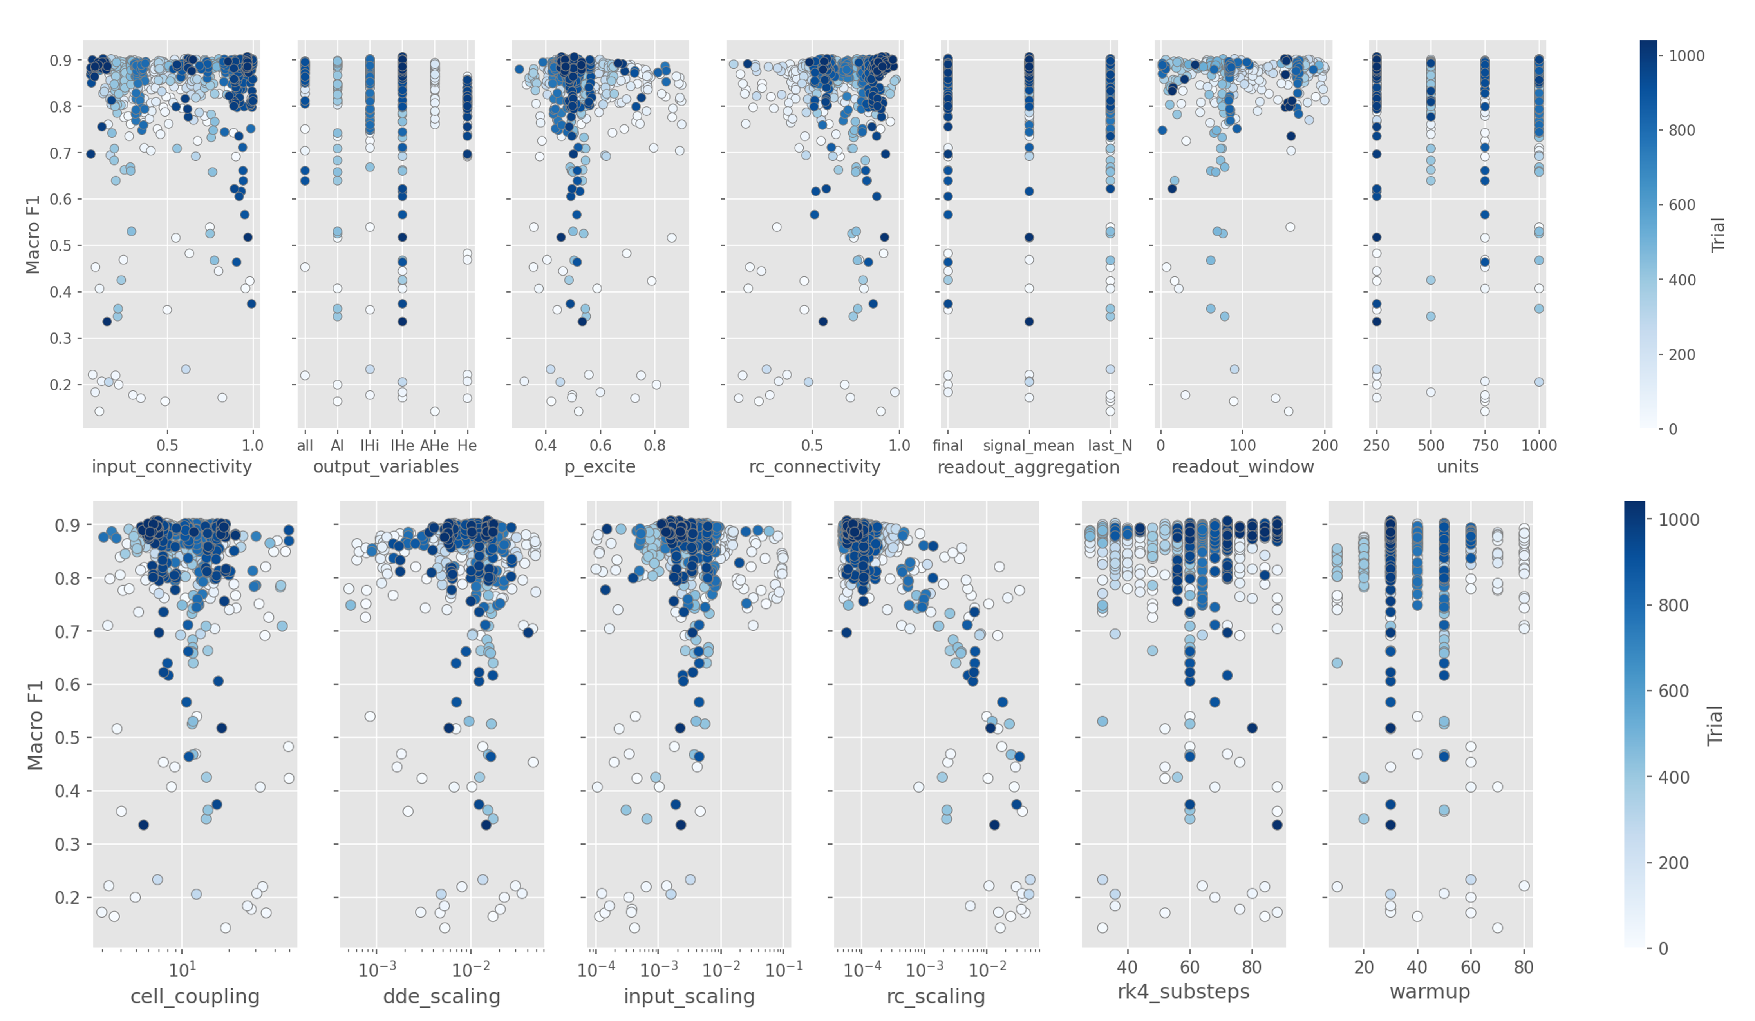
\includegraphics[width=0.95\linewidth]{P2-random-slice.pdf}
    \caption{Phase~2 joint optimization for the random Gaussian topology (P2-random, 800 trials). The random topology converges to a qualitatively different parameter regime than the distance-based topology, with near-full recurrent and input connectivity, higher DDE scaling, and a smaller preferred reservoir size. The upper row summarizes topology, input, and readout parameters; the lower row summarizes scaling and integration parameters.}\label{fig:P2-random}
\end{figure}

\subsection{Topology Comparison Under Robust Evaluation}

On single-fold evaluation during optimization, P2-random marginally outperformed P2-distance ($F_1 = 0.907$ vs.\ $0.905$). However, under five-fold stratified cross-validation, the distance topology showed superior generalization:

\begin{table}[H]
\centering
\caption{Performance comparison between distance-based (P2-distance) and random Gaussian (P2-random) topologies. Single-fold values from optimization; five-fold values from held-out evaluation.}\label{tab:topology-comparison}\small % chktex 24
\begin{tabular}{lcc}
\toprule
Metric & Distance (P2-distance) & Random (P2-random) \\
\midrule
Single-fold $F_1$ (optimization) & 0.905 & 0.907 \\
Five-fold $F_1$ (mean $\pm$ std) & $0.890 \pm 0.007$ & $0.881 \pm 0.013$ \\
Five-fold accuracy & 0.890 & 0.880 \\
Five-fold MCC & 0.863 & 0.851 \\
Fivefold $\kappa$ & 0.862 & 0.850 \tabularnewline
\bottomrule
\end{tabular}
\end{table}

The reversal of ranking from single-fold to five-fold evaluation indicates that the P2-random best trial was more sensitive to the specific data partition used during optimization. The distance topology provides a structured connectivity prior that constrains the search space in a way that promotes configurations robust to data variability. This finding supports the use of biologically motivated topologies not only for physical plausibility but also for improved statistical generalization.

% ==========================================================
\section{Hyperparameter Optimization --- Phase~3 Final Configuration}
% ==========================================================

Phase~3 evaluated the best Phase~2 distance-topology configuration (P2-distance, trial~416) under two additional experimental settings, both using full five-fold stratified cross-validation.

\subsection{Class Imbalance Study (P3-imbalance)}

A grid search varied the maximum samples per class from $1\times$ (803) to $5\times$ (4015). Each class contributes up to the cap or its available count, whichever is smaller; Fusion (803 total) is the smallest contributor throughout, while Supraventricular reaches its natural limit of 2\,779 at $4\times$ and above. Stratified five-fold CV preserves these unequal class proportions in each fold. Performance increased monotonically with dataset size, reaching a headline five-fold macro F1-score of $0.920 \pm 0.005$ at $5\times$ (Table~2 of the main article).

\subsection{Binary Classification (P3-binary)}

Binary classification (Normal vs.\ Arrhythmia) was evaluated using the same P2-distance reservoir parameters. Non-Normal classes were merged into a single Arrhythmia category and downsampled to match the minority class size. Using the readout-selection subset ($4{,}015$ instances, matching the balanced five-class dataset size) with KNN ($k = 4$, the pre-readout baseline), the model achieved a five-fold macro F1-score of $0.931 \pm 0.004$. This value is the inherited P3-binary baseline from the direct five-fold rerun; the slightly lower KNN score reported later for P4-readout-binary ($0.929$) comes from the separate frozen-state readout search on the same subset, where re-optimized KNN hyperparameters did not surpass the inherited baseline. Phase~4 readout optimization on this subset selected random forest as the best binary classifier ($F_1 = 0.933$). The final headline binary result was then obtained by retraining with the selected readout on the full balanced dataset ($18{,}857$ instances per class; $37{,}714$ total CV pool; ${\approx}15{,}086$ training instances per fold), yielding $F_1 = 0.961 \pm 0.002$ (Table~\ref{tab:headline-summary}).

% ==========================================================
\section{Hyperparameter Optimization --- Phase~4 Readout Optimization}
% ==========================================================

Phase~4 optimized the readout classifier on frozen reservoir states generated from the best configurations of Phases 2--3. Reservoir dynamics were computed once and cached, so only the readout algorithm and its hyperparameters were varied.

\subsection{Methodology}

Seven classifier families were evaluated: $K$-nearest neighbors (KNN), gradient boosting (GB), random forest (RF), ridge classifier, logistic regression (LR), support vector machine (SVM), and decision tree (DT), each with family-specific hyperparameter search ranges. Optuna TPE search was used with five-fold cross-validated macro F1-score as the objective. Because the states were frozen, these studies were computationally inexpensive relative to reservoir simulation.

\subsection{Balanced Five-Class Readout (P4-readout-balanced)}

A total of 914 TPE trials were evaluated across all classifier families. Table~\ref{tab:P4-readout-balanced} reports the best F1-score per classifier.

\begin{table}[H]
    \centering
    \caption{Best macro F1-score per classifier for the balanced five-class readout study (914 trials, fivefold CV on frozen reservoir states).}
    \label{tab:P4-readout-balanced}
    \small
    \begin{tabular}{lcc}
        \toprule
        Classifier & Best F1 & Key Hyperparameters \\
        \midrule
        KNN & \textbf{0.891} & $k = 4$, weights = distance, $p = 1.03$ \\
        Gradient Boosting & 0.878 & $n_{\mathrm{est}} = 478$, lr $= 0.83$, loss = exponential \\
        Random Forest & 0.875 & $n_{\mathrm{est}} = 248$, criterion = log\_loss \\
        Ridge Classifier & 0.853 & $\alpha = 70.0$, solver = svd \\
        Logistic Regression & 0.844 & $C = 0.39$, solver = liblinear \\
        SVM & 0.805 & $C = 8 \times 10^{-5}$, kernel = linear \\
        Decision Tree & 0.812 & criterion = log\_loss, leaf $= 5$ \\
        \bottomrule
    \end{tabular}
\end{table}

KNN with $k = 4$ (distance-weighted) achieved the highest F1-score.

\subsection{Unbalanced Five-Class Readout (P4-readout-unbalanced)}

A total of 747 TPE trials were evaluated on frozen states from the $5\times$ unbalanced configuration.

\begin{table}[H]
    \centering
    \caption{Best macro F1-score per classifier for the unbalanced five-class readout study (P4-readout-unbalanced, 747 trials).}\label{tab:P4-readout-unbalanced}
    \small
    \begin{tabular}{lcc}
        \toprule
        Classifier & Best F1 & Key Hyperparameters \\
        \midrule
        KNN & \textbf{0.920} & $k = 1$, weights = uniform, $p = 1.61$ \\
        Random Forest & 0.917 & $n_{\mathrm{est}} = 215$, criterion = entropy \\
        Gradient Boosting & 0.895 & $n_{\mathrm{est}} = 107$, lr $= 0.24$ \\
        Ridge Classifier & 0.891 & $\alpha = 2.8$ \\
        Logistic Regression & 0.879 & $C = 8.7$, solver = saga \\
        Decision Tree & 0.871 & criterion = log\_loss, leaf $= 3$ \\
        SVM & 0.839 & $C = 9 \times 10^{-4}$, kernel = poly, degree $= 2$ \\
        \bottomrule
    \end{tabular}
\end{table}

KNN again dominated, with $k = 1$ and uniform weighting.

\subsection{Binary Readout (P4-readout-binary)}

A total of 1013 TPE trials were evaluated on frozen states from the binary classification task. To ensure a fair comparison with the five-class readout studies, readout selection was performed on a $4{,}015$-instance subset (matching the balanced five-class dataset size) rather than the full binary dataset ($37{,}714$ instances).

\begin{table}[H]
    \centering
    \caption{Best macro F1-score per classifier for the binary readout study (P4-readout-binary, 1013 trials, evaluated on a $4{,}015$-instance subset). The final headline binary result ($F_1 = 0.961$) was obtained by applying the selected readout to the full balanced dataset.}\label{tab:P4-readout-binary}
    \small
    \begin{tabular}{lcc}
        \toprule
        Classifier & Best F1 & Key Hyperparameters \\
        \midrule
        Random Forest & \textbf{0.933} & $n_{\mathrm{est}} = 285$, criterion = entropy, depth $= 47$ \\
        Gradient Boosting & 0.931 & $n_{\mathrm{est}} = 415$, lr $= 0.41$ \\
        KNN & 0.929 & $k = 3$, weights = distance, $p = 1.73$ \\
        Ridge Classifier & 0.922 & $\alpha = 2.8$, solver = sparse\_cg \\
        Logistic Regression & 0.916 & $C = 1448$, solver = newton-cg \\
        SVM & 0.902 & $C = 2.5$, kernel = poly, degree $= 2$ \\
        Decision Tree & 0.894 & criterion = entropy, leaf $= 1$ \\
        \bottomrule
    \end{tabular}
\end{table}

In contrast to the five-class tasks, random forest outperformed KNN for binary classification ($F_1 = 0.933$ vs.\ $0.929$). Readout selection was performed on a $4{,}015$-instance subset for parity with the five-class studies; the final headline binary result ($F_1 = 0.961$) was obtained by applying the selected readout to the full balanced dataset ($37{,}714$ instances).

\begin{figure}[H]
    \centering
    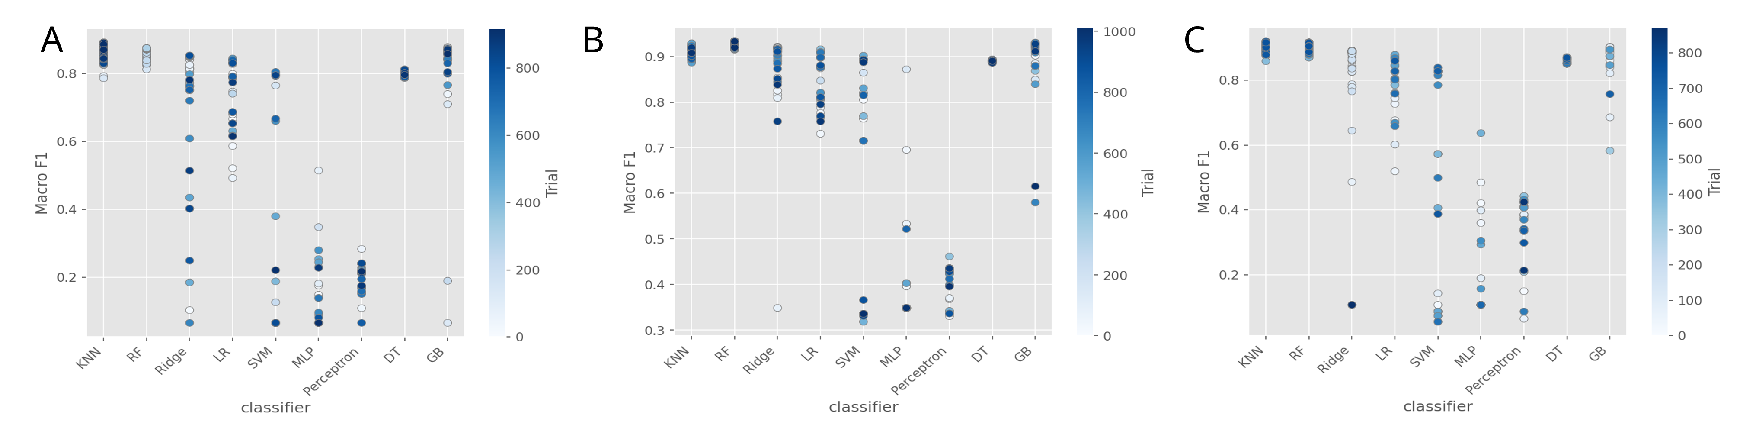
\includegraphics[width=0.95\linewidth]{headline-classifiers-slice.pdf}
    \caption{Phase~4 readout optimization slice plots across all three headline tasks. Each panel shows macro F1 vs.\ classifier family and its hyperparameters. (A)~Balanced five-class: KNN with distance weighting dominates. (B)~Binary: random forest and gradient boosting overtake distance-based methods. (C)~Unbalanced five-class: KNN with uniform $k = 1$ is the top performer.}\label{fig:P4-readout-all}
\end{figure}

% ==========================================================
\section{Final Headline Metrics}
% ==========================================================

This section reports the complete five-fold cross-validation metrics for all headline results.

\subsection{Unbalanced Five-Class Classification}

Using the $5\times$ unbalanced configuration ($N = 1000$, KNN $k = 1$, uniform weighting), the model achieved a macro F1-score of $0.920 \pm 0.005$ (Table~\ref{tab:unbalanced-metrics-si}).

\begin{table}[H]
    \centering
    \caption{Per-class classification metrics for the unbalanced five-class task (mean $\pm$ std across five folds).}\label{tab:unbalanced-metrics-si}
    \small
    \begin{tabular}{lccc}
        \toprule
        Class & Precision & Recall & F1-score \\
        \midrule
        Normal (N) & $0.887 \pm 0.005$ & $0.902 \pm 0.013$ & $0.894 \pm 0.009$ \\
        Supraventricular (S) & $0.877 \pm 0.013$ & $0.863 \pm 0.014$ & $0.870 \pm 0.009$ \\
        Ventricular (V) & $0.944 \pm 0.006$ & $0.933 \pm 0.009$ & $0.939 \pm 0.006$ \\
        Fusion (F) & $0.814 \pm 0.009$ & $0.827 \pm 0.052$ & $0.819 \pm 0.027$ \\
        Unknown (Q) & $0.979 \pm 0.004$ & $0.981 \pm 0.006$ & $0.980 \pm 0.004$ \\
        \midrule
        Macro avg. & & & $0.920 \pm 0.005$ \\
        \bottomrule
    \end{tabular}
\end{table}

\subsection{Summary of All Headline Results}

Table~\ref{tab:headline-summary} provides a consolidated view of all headline classification results.

\begin{table}[H]
    \centering
    \caption{Summary of headline classification results across all evaluated tasks. All values from five-fold stratified cross-validation ($N = 1000$ distance-based topology unless noted). Wall time is total end-to-end duration with five parallel folds on Host~1.}\label{tab:headline-summary}
    \small
    \begin{tabular}{lcccccc}
        \toprule
        Task & F1 (mean $\pm$ std) & Accuracy & MCC & $\kappa$ & Readout & Wall time \\
        \midrule
        Balanced 5-class & $0.890 \pm 0.007$ & 0.890 & 0.863 & 0.862 & KNN ($k\!=\!4$) & ${\sim}5$\,min \\
        ESN baseline$^{*}$ & $0.878 \pm 0.014$ & 0.875 & 0.846 & 0.843 & Ridge & ${\sim}2$\,min \\
        Raw baseline (bal.)$^{\ddagger}$ & $0.886 \pm 0.013$ & 0.885 & 0.857 & 0.857 & SVM (poly) & ${\sim}6$\,s \\
        Unbalanced 5-class & $0.920 \pm 0.005$ & 0.920 & 0.896 & 0.896 & KNN ($k\!=\!1$) & ${\sim}22$\,min \\
        Raw baseline (unbal.)$^{\ddagger}$ & $0.916 \pm 0.002$ & 0.932 & 0.911 & 0.911 & SVM (RBF) & ${\sim}52$\,s \\
        Binary & $0.961 \pm 0.002$ & 0.961 & 0.923 & 0.922 & RF ($n\!=\!285$) & ${\sim}52$\,min \\
        Raw baseline (bin.)$^{\ddagger}$ & $0.933 \pm 0.004$ & 0.933 & 0.867 & 0.866 & SVM (RBF) & ${\sim}12$\,s \\
        Random topology$^{\dagger}$ & $0.881 \pm 0.013$ & 0.880 & 0.851 & 0.850 & KNN ($k\!=\!1$) & ${\sim}5$\,h \\
        \bottomrule
        \multicolumn{7}{l}{\parbox{0.92\textwidth}{\footnotesize $^{*}$Standard leaky ESN baseline optimized under the same balanced five-class preprocessing, macro-F1 objective, and frozen-state readout-selection workflow as the BioReservoir. $^{\dagger}$Balanced five-class task with a random Gaussian connectivity matrix ($N = 250$; see Table~\ref{tab:topology-comparison}). The elevated wall time reflects the near-full recurrent connectivity (\texttt{rc\_connectivity} $= 0.90$) selected by the optimizer, yielding a dense $250 \times 250$ weight matrix that increases recurrent matrix-vector product cost per timestep compared to the sparse distance-based kernel. $^{\ddagger}$No-reservoir baseline: classifiers trained directly on raw z-scored 187-d ECG features (see Section~\ref{sec:si-baseline}). Binary baseline uses a $4{,}015$-instance subset matching the reservoir readout-selection pool; the headline binary result ($F_1 = 0.961$) used the full balanced dataset.}} \\
    \end{tabular}
\end{table}

% ====================================================================
\section{Ablation Studies}\label{sec:si_ablation} % chktex 8
% ====================================================================

To quantify the contribution of individual dynamical features to classification performance, we conducted three ablation experiments on the balanced five-class pipeline.
Each condition modified a single aspect of the optimized reservoir (P2-distance best trial parameters) while holding all other hyperparameters fixed, then evaluated performance using the same five-fold cross-validation protocol.
Below we summarize the experimental conditions. The main text (Section~2.8) presents the headline results and interpretation.

\begin{enumerate}
  \item \textbf{Coupling ablation} ($\alpha_{\mathrm{rc}} = 0$): the recurrent coupling scaling was set to zero so that each oscillator evolved independently, driven only by the input signal.
        This tests whether inter-node interactions contribute information beyond what isolated nonlinear integrators provide.
  \item \textbf{Delay ablation} ($\tau = 0$): the transcriptional delay was set to zero, converting the delay differential equation system into an ordinary differential equation system.
        This removes the history-dependent dynamics and tests whether the delayed feedback loop is necessary for temporal feature extraction.
  \item \textbf{Input scrambling}: for each ECG instance independently, the 187 input timesteps were randomly permuted before being presented to the reservoir.
        This preserves amplitude distributions and per-instance summary statistics while destroying all temporal structure, serving as a negative control for genuine sequential processing.
\end{enumerate}

In addition, a \textbf{topology statistical test} compared the existing distance-based (r1a) and random (r1b) fold-level results using paired tests.

Table~\ref{tab:si-ablation-per-fold} reports per-fold macro F1 scores for each condition.

\begin{table}[H]
\centering
\caption{Per-fold macro F1 scores for the ablation experiments on balanced five-class classification. The baseline is the full optimized model (P2-distance best trial).}\label{tab:si-ablation-per-fold}
\small
\begin{tabular}{lccccccc}
\toprule
& \multicolumn{5}{c}{Fold} & & \\
\cmidrule(lr){2-6}
Condition & 0 & 1 & 2 & 3 & 4 & Mean & Std \\
\midrule
Full model (baseline) & 0.896 & 0.893 & 0.885 & 0.880 & 0.895 & 0.890 & 0.007 \\
No coupling ($\alpha_{\mathrm{rc}} = 0$) & 0.809 & 0.819 & 0.817 & 0.799 & 0.820 & 0.813 & 0.009 \\
No delay ($\tau = 0$) & 0.805 & 0.801 & 0.812 & 0.799 & 0.829 & 0.809 & 0.012 \\
Scrambled input & 0.195 & 0.213 & 0.203 & 0.207 & 0.211 & 0.206 & 0.007 \\
\bottomrule
\end{tabular}
\end{table}

\subsection{Topology Statistical Test}

A formal paired comparison of the distance-based and random topology fold results yielded the following:
\begin{itemize}
  \item Distance-based: $F_1 = 0.890 \pm 0.007$; Random: $F_1 = 0.881 \pm 0.015$.
  \item Paired $t$-test: $t(4) = 1.46$, $p = 0.217$.
  \item Wilcoxon signed-rank test: $W = 3.0$, $p = 0.3125$.
  \item Cohen's $d = 0.65$; 95\% CI for the mean difference: $[-0.008, +0.027]$.
\end{itemize}
The moderate effect size (Cohen's $d = 0.65$) is consistent with a real but small advantage for the distance topology; however, statistical significance is not reached with five folds, and the confidence interval spans zero.
A definitive conclusion would require a larger number of independent folds or repeated-measures designs.

% ====================================================================
\section{Cell-to-Cell Kinetic Heterogeneity}\label{sec:heterogeneity}
% ====================================================================

Real bacterial populations exhibit substantial cell-to-cell variability in gene expression and protein abundance.\cite{Elowitz2002,Taniguchi2010,Raj2008}
To assess whether the reservoir's classification performance is robust to such biological noise, we conducted a systematic sweep over kinetic-parameter heterogeneity.
For each trial, every reservoir node drew its 13 intracellular kinetic rate constants (transcription, translation, enzymatic degradation, and Hill-function parameters) independently from log-normal distributions:
%
\begin{equation}
  \theta_i \sim \theta_0 \cdot \exp\!\bigl(\mathcal{N}(0,\,\sigma^2)\bigr), \qquad \sigma = \sqrt{\ln(1 + \mathrm{CV}^2)},
\end{equation}
%
where $\theta_0$ denotes the nominal Danino et~al.\cite{Danino2010} value and $i$ indexes reservoir nodes.
Colony-level parameters (cell density fraction~$d$, extracellular decay~$\mu$, and derived dilution rate) were held fixed, as they represent environmental or population-scale quantities rather than single-cell properties.

All reservoir hyperparameters (scaling coefficients, topology, coupling strength, noise levels) were fixed at the values optimized under homogeneous conditions (P2-distance best trial; Table~\ref{tab:P2-distance-best}), with \emph{no re-tuning} for any heterogeneity level.
This design tests inherent robustness rather than re-optimized performance.

The study swept eight CV levels ($0, 0.025, 0.05, 0.1, 0.15, 0.2, 0.3, 0.5$) crossed with five independent random seeds for the parameter draws, yielding 40 grid points evaluated on a single fold of the balanced five-class task ($N = 1000$ nodes, distance-based topology).
Of these, 36 trials completed successfully; the four missing grid points are distributed across different CV levels and do not affect the conclusions.

\subsection{Reservoir Robustness}

Figure~\ref{fig:heterogeneity} summarizes the results.
Within the low-to-moderate heterogeneity range ($\mathrm{CV} \leq 0.1$), classification performance was preserved or slightly improved relative to the single-fold homogeneous baseline ($F_1 = 0.887$): mean $F_1 = 0.890$ at $\mathrm{CV} = 0.025$, $0.893$ at $\mathrm{CV} = 0.05$, and $0.894$ at $\mathrm{CV} = 0.1$.
These values are single-fold macro F1 scores from the fixed balanced evaluation fold used for the heterogeneity sweep and are therefore not directly comparable to the five-fold headline macro F1-score of $0.890$ reported in the main text.
We interpret this small uplift conservatively as evidence that modest heterogeneity does not damage the reservoir, rather than as proof that heterogeneity is intrinsically beneficial.

At higher CV levels, performance degraded gracefully: $F_1 = 0.866$ at $\mathrm{CV} = 0.2$, $0.862$ at $\mathrm{CV} = 0.3$, and $0.848$ at $\mathrm{CV} = 0.5$.
Even in the worst case ($\mathrm{CV} = 0.5$), the decline from baseline was only 4.4\%, and the system never collapsed.

\begin{figure}[H]
    \centering
    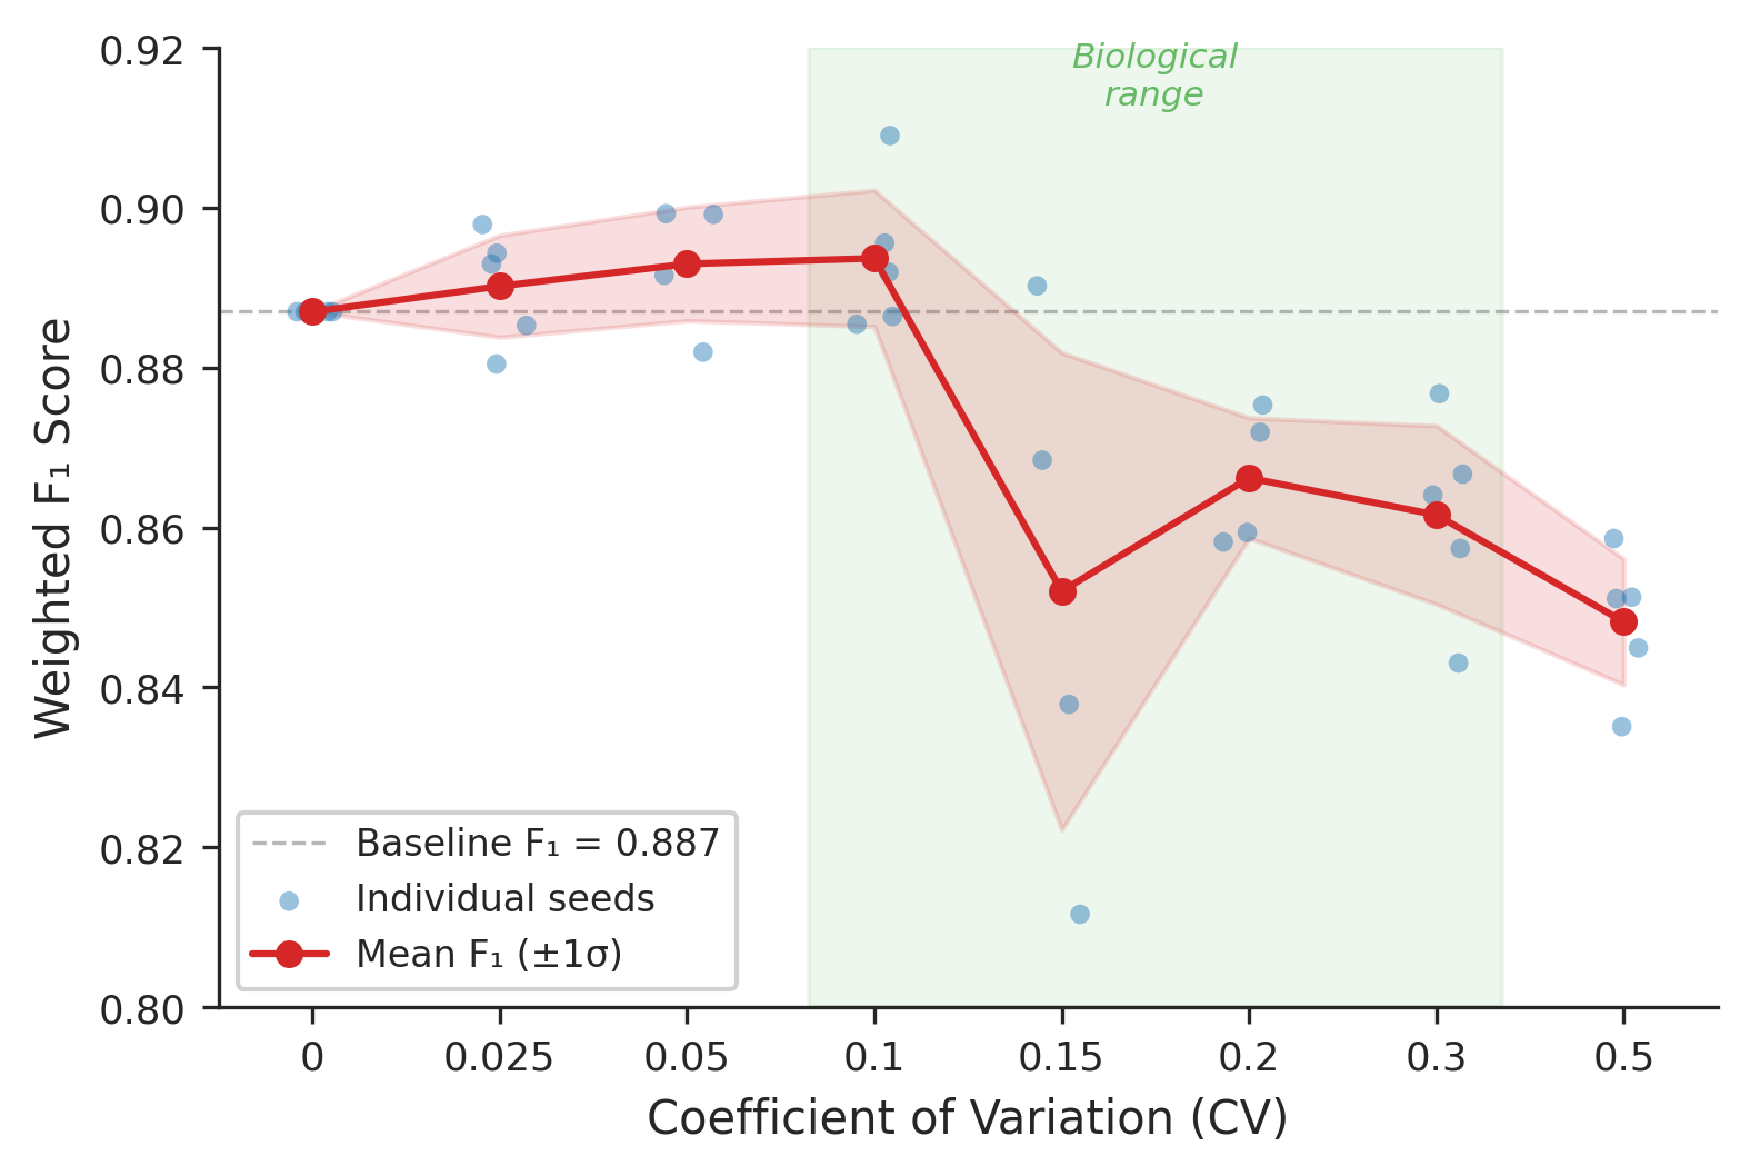
\includegraphics[width=0.85\linewidth]{heterogeneity_robustness.pdf}
    \caption{Macro F$_1$-score as a function of per-node kinetic parameter heterogeneity (coefficient of variation, CV).
    Red line: mean across five independent random seeds; shaded band: $\pm 1\sigma$.
    Blue dots: individual seed realizations.
    Green shading marks a representative low-to-moderate heterogeneity band ($\mathrm{CV} = 0.1$--$0.3$).
    The dashed line indicates the single-fold homogeneous baseline ($F_1 = 0.887$).
    All trials used the hyperparameters optimized under homogeneous conditions, with no re-tuning. Because the heterogeneity sweep uses a balanced evaluation fold with equal class support, macro and weighted F$_1$ are numerically identical here; we report macro F$_1$ for consistency with the main text.}\label{fig:heterogeneity}
\end{figure}

\subsection{Per-Class Breakdown}

Table~\ref{tab:heterogeneity-per-class} shows that the degradation is not uniform across classes.
Class~Q (Unknown), which has the most morphologically distinct waveform, was essentially invariant ($F_1$: $0.969 \to 0.957$ from $\mathrm{CV} = 0$ to $0.5$).
The decline concentrated on morphologically similar classes~N (Normal) and~S (Supraventricular), where fine-grained discrimination relies on subtle temporal features that are most sensitive to altered oscillator dynamics.

\begin{table}[H]
    \centering
    \caption{Per-class F$_1$-score (mean across seeds) as a function of kinetic-parameter heterogeneity.
    Class labels follow the AAMI standard: N~(Normal), S~(Supraventricular), V~(Ventricular premature), F~(Fusion), Q~(Unknown/paced).}\label{tab:heterogeneity-per-class}
    \small
    \begin{tabular}{ccccccccc}
        \toprule
        & \multicolumn{8}{c}{Coefficient of Variation (CV)} \\
        \cmidrule(lr){2-9}
        Class & 0.0 & 0.025 & 0.05 & 0.1 & 0.15 & 0.2 & 0.3 & 0.5 \\
        \midrule
        N & 0.806 & 0.813 & 0.827 & 0.830 & 0.759 & 0.797 & 0.787 & 0.765 \\
        S & 0.855 & 0.867 & 0.864 & 0.872 & 0.826 & 0.847 & 0.836 & 0.811 \\
        V & 0.909 & 0.907 & 0.905 & 0.903 & 0.864 & 0.867 & 0.861 & 0.855 \\
        F & 0.897 & 0.900 & 0.895 & 0.891 & 0.858 & 0.864 & 0.867 & 0.855 \\
        Q & 0.969 & 0.964 & 0.975 & 0.974 & 0.955 & 0.957 & 0.958 & 0.957 \\
        \midrule
        \textbf{Macro} & \textbf{0.887} & \textbf{0.890} & \textbf{0.893} & \textbf{0.894} & \textbf{0.852} & \textbf{0.866} & \textbf{0.862} & \textbf{0.848} \\
        \bottomrule
    \end{tabular}
\end{table}

% ====================================================================
\section{No-Reservoir Baseline}\label{sec:si-baseline}
% ====================================================================

To quantify the contribution of the reservoir transformation independently of the readout classifier, we trained the same classifier families used in Phase~4 readout optimization---plus MLP and perceptron---directly on the raw z-scored 187-dimensional ECG feature vectors, bypassing the reservoir entirely. Three studies were conducted:

\begin{enumerate}
  \item \textbf{B1-baseline} (balanced five-class): $4{,}015$ instances, same balanced dataset and class distribution as Phase~4 readout-balanced.
  \item \textbf{B2-baseline-unbalanced} (unbalanced five-class): per-class cap of $4{,}015$ with the full available pool (${\sim}50{,}000$ instances), matching the $5\times$ imbalance configuration.
  \item \textbf{B3-baseline-binary} (binary Normal vs.\ Arrhythmia): $4{,}015$ balanced binary instances, matching the readout-selection subset used for binary readout optimization.
\end{enumerate}

All three studies used the same evaluation methodology as the Phase~4 readout studies: five-fold stratified cross-validation with per-fold noise augmentation, per-sequence z-score normalization, and macro-F1 as the optimization objective. The only change was the input representation: raw 187-dimensional ECG vectors rather than frozen reservoir states.

\subsection{Balanced Five-Class Baseline (B1-baseline)}

A total of 376 TPE trials were completed across nine classifier families. Table~\ref{tab:B1-baseline} reports the best F1-score per classifier.

\begin{table}[H]
    \centering
    \caption{Best macro F1-score per classifier for the balanced five-class no-reservoir baseline (B1-baseline, 376 completed trials, five-fold CV on raw z-scored ECG features).}
    \label{tab:B1-baseline}
    \small
    \begin{tabular}{lc}
        \toprule
        Classifier & Best F1 \\
        \midrule
        SVM (poly) & \textbf{0.886} \\
        MLP & 0.881 \\
        Random Forest & 0.880 \\
        KNN & 0.869 \\
        Gradient Boosting & 0.864 \\
        Decision Tree & 0.820 \\
        Logistic Regression & 0.761 \\
        Ridge Classifier & 0.732 \\
        Perceptron & 0.682 \\
        \bottomrule
    \end{tabular}
\end{table}

SVM with a polynomial kernel achieved the highest F1-score on raw features. The classifier ranking differs substantially from the reservoir-state ranking (Table~\ref{tab:P4-readout-balanced}), motivating the cross-task summary below.

\subsection{Unbalanced Five-Class Baseline (B2-baseline-unbalanced)}

A total of 435 TPE trials were completed.

\begin{table}[H]
    \centering
    \caption{Best macro F1-score per classifier for the unbalanced five-class no-reservoir baseline (B2-baseline-unbalanced, 435 completed trials).}
    \label{tab:B2-baseline}
    \small
    \begin{tabular}{lc}
        \toprule
        Classifier & Best F1 \\
        \midrule
        SVM (RBF) & \textbf{0.916} \\
        MLP & 0.914 \\
        Random Forest & 0.905 \\
        KNN & 0.900 \\
        Gradient Boosting & 0.889 \\
        Decision Tree & 0.855 \\
        Logistic Regression & 0.742 \\
        Ridge Classifier & 0.732 \\
        Perceptron & 0.668 \\
        \bottomrule
    \end{tabular}
\end{table}

The unbalanced task shows a similar pattern, with SVM-RBF and MLP performing strongest on raw features.

\subsection{Binary Baseline (B3-baseline-binary)}

A total of 480 TPE trials were completed.

\begin{table}[H]
    \centering
    \caption{Best macro F1-score per classifier for the binary no-reservoir baseline (B3-baseline-binary, 480 completed trials, $4{,}015$-instance balanced subset).}
    \label{tab:B3-baseline}
    \small
    \begin{tabular}{lc}
        \toprule
        Classifier & Best F1 \\
        \midrule
        SVM (RBF) & \textbf{0.933} \\
        KNN & 0.931 \\
        MLP & 0.930 \\
        Random Forest & 0.926 \\
        Gradient Boosting & 0.926 \\
        Decision Tree & 0.892 \\
        Logistic Regression & 0.812 \\
        Ridge Classifier & 0.807 \\
        Perceptron & 0.764 \\
        \bottomrule
    \end{tabular}
\end{table}

For binary classification, several classifier families reach a similar performance ceiling on both raw features and reservoir states.

\subsection{Cross-Task Summary: Reservoir vs.\ Raw Features}

Table~\ref{tab:reservoir-vs-raw-summary} summarizes the per-classifier comparison across all three tasks, highlighting the reservoir's effect on linear vs.\ nonlinear readouts.

\begin{table}[H]
    \centering
    \caption{Macro F1-score improvement ($\Delta$) from reservoir states over raw features, per classifier and task. Positive values indicate the reservoir transformation improved performance; negative values indicate raw features were superior for that classifier. Classifiers are ordered by mean $\Delta$ across tasks.}
    \label{tab:reservoir-vs-raw-summary}
    \small
    \begin{tabular}{lcccccc}
        \toprule
        & \multicolumn{2}{c}{Balanced 5-class} & \multicolumn{2}{c}{Unbalanced 5-class} & \multicolumn{2}{c}{Binary} \\
        \cmidrule(lr){2-3} \cmidrule(lr){4-5} \cmidrule(lr){6-7}
        Classifier & $\Delta$ & Raw & $\Delta$ & Raw & $\Delta$ & Raw \\
        \midrule
        Ridge      & $+0.121$ & 0.732 & $+0.159$ & 0.732 & $+0.115$ & 0.807 \\
        LR         & $+0.083$ & 0.761 & $+0.137$ & 0.742 & $+0.104$ & 0.812 \\
        KNN        & $+0.022$ & 0.869 & $+0.020$ & 0.900 & $-0.003$ & 0.931 \\
        GB         & $+0.014$ & 0.864 & $+0.040$ & 0.863 & $+0.005$ & 0.926 \\
        RF         & $-0.005$ & 0.880 & $+0.020$ & 0.897 & $+0.007$ & 0.926 \\
        DT         & $-0.008$ & 0.820 & $+0.016$ & 0.855 & $+0.002$ & 0.892 \\
        SVM        & $-0.081$ & 0.886 & $-0.077$ & 0.916 & $-0.031$ & 0.933 \\
        MLP        & $-0.366$ & 0.881 & $-0.276$ & 0.913 & $-0.058$ & 0.930 \\
        \bottomrule
    \end{tabular}
\end{table}

The pattern is consistent across all three tasks: the reservoir transformation provides substantial improvements for linear and simple readouts (ridge: $+0.12$ to $+0.16$; LR: $+0.08$ to $+0.14$), modest improvements for instance-based methods (KNN, RF), and consistent degradation for classifiers that perform their own nonlinear feature mapping (SVM, MLP). This demonstrates that the reservoir is performing a genuine nonlinear transformation of the input space---one that is well-aligned with the requirements of simple readouts but redundant with the internal representations learned by complex classifiers. KNN and GB on the unbalanced task have fewer completed trials than other families due to their long per-trial runtimes on the larger dataset, but the available data are consistent with the overall pattern.

\bibliography{references}

\end{document}
